\documentclass[fontsize=12pt,paper=A4,pagesize,DIV=calc,BCOR=1cm]{scrreprt}
\usepackage{lmodern}
\usepackage{setspace}
\usepackage[utf8]{inputenc}
\usepackage[T1]{fontenc}
\usepackage[ngerman]{babel}
\usepackage{graphicx}
\usepackage[table]{xcolor}
\usepackage{hyperref}
\usepackage{float}
\usepackage{fancyhdr}
\usepackage{pifont}

\usepackage[babel,german=guillemets]{csquotes}
\usepackage[backend=biber,style=alphabetic,bibstyle=alphabetic, block=space, url=true]{biblatex}
\addbibresource{references.bib}
\usepackage[paper=a4paper,left=25mm,right=10mm,top=20mm,bottom=25mm]{geometry}
\usepackage[Bjornstrup]{fncychap}
\usepackage{listings} 
\normalfont

\pagestyle{fancyplain}

\newcommand{\mytitle}{Exposé}
\newcommand{\mops}{\textit{{\large M}\textsc{op}{\large S} }}
\newcommand{\me}{Christopher \textsc{Kruczek}}

\renewcommand{\chaptermark}[1]{\markboth{#1}{}}
\renewcommand{\sectionmark}[1]{\markright{#1}}



\lhead[\fancyplain{}{\leftmark}]         {\fancyplain{}{\leftmark}}
\chead[\fancyplain{}{\mytitle}]                 {\fancyplain{}{\mytitle}}
\rhead[\fancyplain{}{\rightmark}]       {\fancyplain{}{\rightmark}}
\lfoot[\fancyplain{}{}]                 {\fancyplain{\me}{\me}}
\cfoot[\fancyplain{\today}{}]         {\fancyplain{\today}{\today}}
\rfoot[\fancyplain{\thepage}]  {\fancyplain{\thepage}{\thepage}}

% Bjornstrup chapter formating
\ChNumVar{\fontsize{76}{80}\usefont{OT1}{pzc}{m}{n}\selectfont}
\ChTitleVar{\raggedright\Huge\bf}


\begin{document}

\onehalfspacing

\begin{titlepage}
	\begin{center} 
		\vspace*{2 cm}
		\textsc{\LARGE \mytitle}
		\rule{\textwidth}{0.4pt} \\[1.5cm]
		\textsc{\Large Bachelorarbeit zur Erlangung des Bachelor of Science f\"ur Angewandte Informatik}\\[1.5cm]
			
			 Fachhochschule für Technik und Wirtschaft Berlin\\
Fachbereich Wirtschaftswissenschaften II\\
Studiengang Angewandte Informatik\\[1cm]			
		\vspace{3cm}
	\end{center}

\begin{center}
\begin{tabular}[h!]{l l}
1. Betreuer: & Prof. Dr. Frank \textsc{Bauern\"oppel}\\
2. Betreuer: & Prof. Dr. Burkhard \textsc{Messer}\\[2cm]
Eingereicht durch: & Christopher \textsc{Kruczek}
\end{tabular}
\end{center}

	\vfill
	\center {\today}
\end{titlepage}
% just force a empty page after the titlepage
\newpage
\thispagestyle{empty}
\mbox{}

\tableofcontents
\pagenumbering{roman}
\listoftables
\listoffigures
\lstlistoflistings
\pagenumbering{arabic}
\chapter{Einleitung}
\begin{quote}
\blockquote{\textit{Der Entwurf eines Betriebssystem erfordert eher ein ingeneursm\"a\ss iges Vorgehen, als ein exaktes wissenschaftliches. Es ist schwieriger, klaere Ziele zu definieren und diese zu erreichen.}}\parencite[911]{os}
\end{quote}
Mit dieser Aussage leitet Tanenbaum das Thema der Entwicklung eines Betriebssystem ein. Und genau mit dieser Frage soll diese Bachelorarbeit eingeleitet werden. Was sollen also die Ziele dieser Bachelorarbeit sein?\\\\
Das Betriebssystem was im folgenden vorgestellt wird tr\"agt den Akronymnamen \mops - \textbf{M}ini \textbf{Op}erating \textbf{S}ystem und soll seinen Haupteinsatzzweck im Lehrbereich der HTW-Berlin, f\"ur den Studiengang Angewandte Informatik und Wirtschaftsinformatik, finden.\\ \\
Die Entwicklung eines Betriebssystems bringt viele Schwierigkeiten und Herausforderungen mit sich. Eine der Schwierigkeiten ist die Handhabung mit Embedded Systems. Hier zeigt \mops wie man mit einem verh\"altnism\"a\ss ig kleinen Prozessor eine stabile L\"osung erarbeiten kann. Eine weitere Schwierigkeit in diesem Bereich stellt die Benutzung der vorhander Hardware dar. Das hei\ss t z.B. wie wird der Timer konfiguriert, an welche Stelle im RAM muss er geladen oder wie k\"onnen die Ticks behandelt werden. Weiterhin werden Komponenten wie die Serielle Schnittstelle zwischen Tastatur und Monitor beleuchtet. Hier wird eine gezeigt wie man eine Eingabe von der Tastatur abfangen kann, welches Hardwareteil dazu konfiguriert werden muss und wie die Daten auf dem Monitor angezeigt werden k\"onnen. Aber auch der Punkt der Interrupts kommt in diesem Konzept nicht zu kurz. Was bedeuten Interrupts? Wie m\"ussen sie konfiguriert werden? Welche Interrupthandler werden ben\"otigt?\\ Neben all diesen Aspekten stellen Embedded Systems wie z.B. Mobil Telefone, Drucker, Kaffeemaschinen, Tablets den Entwickler vor gro\ss e Herausforderungen was die Thematik Prozessmanagment und Scheduling angeht. Deshalb werden diese Aspekte besonders beleuchtet. Das bedeudet es gibt tiefe Einblicke in das Thema - Laden einens Prozesses -, - Starten eines Prozesses -, - Wechsel zwischen den Prozessen - und vieles mehr. Um der n\"achsten Generation von Informatikern einen leichten Einstieg in dieses Thema zu bieten ist diese Bachelorarbeit entstanden. Sie dient als Anschauungsmaterial und besch\"aftigt sich mit den Grundlagen der Betriebssystementwicklung in Embedded Systemen. Zudem soll die Arbeit den zuk\"unftigen Projektteilnehmern die Angst vor der Betriebssystementwicklung nehmen. \\
Im Rahmen des Projektes \textbf{FOCOS - Family of configurated operating systems}, f\"ur das Sommersemester 2013 begleitet durch Prof. Dr. Messer, soll diese Bachelorarbeit als Basis zur Weiterentwicklung von neuen Komponenten dienen.\\
Da dieses Projekt im Rahmen einer Lehrveranstaltung als Anschauungsmaterial dienen soll, wird besonderer Wert auf Quellcode und Grafische Untermalung im Entwurf gelegt. Zum Abschluss noch ein Zitat von Fernando Corbat\'o, einem der Entwickler von CTSS\footnote{Compatible Time Sharing System} und MULTICS\footnote{Multiplexed Information and Computing Service}
\begin{quote}
\blockquote{\textit{\ldots Meine Definition von Eleganz ist das Erreichen einer gegebenen Funktionalit\"at mit einem Minimum an Mecuhanismen und einem Maximum an Klarheit.}}\parencite[915]{os}
\end{quote}
Dieses Zitat f\"uhrt uns zu einem weiteren wichtigen Punkt in dieser Arbeit. \mops ist auf Einfachheit und \"Uberschaubarkeit ausgelegt. Das hei\ss t es wurde Wert darauf gelegt keine unn\"otigen Sachen zu implementieren.
\chapter{Anforderungskatalog}
\section{Einleitung}
Moderne Betriebssysteme bestehen aus einer Vielzahl an Funktionen und bieten ein umfangreiches Portfolio an M\"oglichkeiten, jedoch muss bei der Entwicklung von Betriebssystemen im Embedded System Bereich darauf geachtet werden, nur die wichtigsten Komponenten zu implementieren und diese wom\"oglich noch hochperformant zu gestalten.\\
In jedem Betriebssytem und auch in \mops gibt es verschiedene Stellen die eine Erkl\"arung und darausfolgend eine Entwicklung bedarfen. Auch in \mops gibt es einen Startmechanismus, viel mehr unter \textit{Booten} bekannt. Hier wurde jedoch begr\"undet der Begriff Startmechanismus gew\"ahlt da kein wirkliches 'hochfahren' statt findet.\\
Des weiteren gibt es auch Interrupts und Quellen die Interrupts aussenden k\"onnen. \mops stellt in der aktuellen Fassung nur zwei Interruptquellen zur Verf\"ugung, zum einen den Timer und die Serielle-Schnittstelle(speziell die Tastatur). Diese Quellen k\"onnen normale und Fast Interrupt Requests aussenden. Je nach Interrupt Request gibt es unterschiedliche Behandlungsmethoden, die sogenannten Interrupthandler.Nat\"urlich gibt es auch unterschiedliche Herangehensweisen wie Interrupts behandelt werden k\"onnen, \mops erledigt diese Aufgabe mit einem Vectored Interrupt Controller.\\
Neben diesen Faktoren gibt es aber auch weitere Mechanismen in einem Betriebssystem die auch \mops pr\"agen. Eines davon sind die Trap-Handler, also Methoden die von einer Trap-Instruktion aufgerufen werden und somit Kernel-Methoden benutzbar machen.\\
Damit ist aber noch kein Betriebssystem funktionsfertig. Es fehlen noch zwei wichtige Mechanismen. Zum einen ist dass, das Threadmanagment also die Verwaltung von User-Programmen. Verwaltung ist hier der Oberbegriff f\"ur die Teilmechanismen des Ladens, Starten und der Wechsel zwischen den Threads.\\
Da \mops voranging im Bereich der Handhelds eingesetzt werden soll ist es f\"ur die Arbeit nicht relevant eine MMU - Memory Managment Unit zu benutzen. F\"ur eine einwandfreie Threadverwaltung ist nat\"urlich auch ein funktionierendes Scheduling notwendig. F\"ur \mops wurde sich entschieden das Round-Robin Verfahren zu benutzen.
%\section{Startmechanismus}
%Der Startvorgang stellt in jedem Betriebssystem eine wichtige Rolle dar. Die M\"oglichkeiten bei \mops stellten sich hier, durch die Non-Existenz von Hardware, als begrenzt dar. Um diese Problematik zu l\"osen, wurde die Entwicklung in einen Emulator verlagert.
%Die g\"angigste Variante seinen Code zu testen, besteht darin eine Datei im passenden Format zu erzeugen und diese beim Start des Emulators zu \"ubergeben. \\
%Das bedeutet in unserem Fall, das s\"amtliche Dateien kompiliert und gelinkt werden m\"ussen.
\section{Interruptquellen und Interrupthandler}
Ein Prozessor muss im Falle eines Interrupts, z.B. ein Reset des Prozessors, IRQ, FIQ, Prefetch Abort, Software Interrupt oder eine undefinierte Aktion, in der Lage sein diese ad\"aquat zu behandeln. Die meist verwandte Vorgehensweise ist es eine Tabelle im Speicher zu definieren, die genau f\"ur diese Zwecke Routinen bereitstellt\parencite[53]{archManI}.\\ Tritt nun eine Interrupt auf, gibt es eine vordefinierte Reihenfolge an Aktionen, die der Prozessor ausf\"uhrt. Damit immer valide Routinen zur Behandlung der Interrupts in dieser Tabelle stehen, muss jene w\"ahrend der Initialisierung des Systems angelegt werden. Was \mops also ben\"otigt ist ein System zur Behandlung und Konfiguration von Interrupts und Interruptquellen.
\section{Vectored Interrupt Controllor}
Dieses System stellt ein Software Interface zum Interruptsystem des Prozessors dar. In Systemen mit klassischen Interrupt Controllern muss die Software sowohl die Herkunft des Interrupt Request, als auch die Interrupt Service Routine ermitteln. Diese Aufgabe \"ubernimmt der VIC nun komplett selbst\"andig.
Die korrekte Behandlung von sowohl Interrupt Requests(IRQ) als auch Fast Interrupt Requests(FIQ) stellen eine wichtige Rolle in Betriebssystemen dar.\\
Hier gibt es zwei unterschiedliche Mechanismen IRQ/FIQ's zu behandeln:

\begin{description}
	\item[Non-Vectored Controller] - Diese Systeme m\"ussen wissen, woher der Request kommt und wo die Routine zur Behandlung des Requests liegt.
	\item[Vectored Interrupt Controller] - Diese Controller vereinen beide oben genannten Fakten, denn sie werden initial mit den Priorit\"aten der Requests und den zugeh\"origen Routinen gef\"ullt und k\"onnen dann zur Laufzeit die passende Routine direkt zur\"uckgeben.
\end{description}
Bei \mops fiel die Entscheidung darauf, die 2. Variante, den Vectored Interrupt Controller, zu implementieren. Die Vorteile werden noch genauer erl\"autert.
\section{Hardware}
Im folgenden wird die Hardware definiert mit der \mops arbeitet. Zum einen sind das Timer und zum anderen die Serielle Schnittstelle.
\subsection{Timer}
Timer stellen wichtige Schl\"usselfaktoren in Betriebssystemen dar. Ihr Hauptzweck ist die periodische Behandlung von Ereignissen und das ansteuern des Schedulers. \\
Der ARM926 stellt vier Timer zur Verf\"ugung, welche sich auf unterschiedlichste Art und Wei\ss e konfigurieren lassen. Die verf\"ugbaren Timer sind hier mit \textit{Timer0 - Timer3} zu benennen\parencite[vgl.][262]{archManI}. Da es f\"ur \mops ausreicht nur auf einen Timer zur\"uck zu greifen wird sp\"ater nur noch von \textit{Timer0} die Rede sein.
\subsection{Serielle Schnittstelle - UART}
Das \textit{Universal Asynchronous Receiver Transmitter} Interface bietet die M\"oglichkeit der seriellen Daten\"ubertragung auf Mikrocontroller. Mittels dieser Schnittstelle ist es unter anderem m\"oglich, die Tastatureingaben abzufragen und Daten auf dem Monitor anzuzeigen. \\
Sicherlich gibt es hier noch speziell daf\"ur ausgelegte Ger\"ate, wie z.B \textit{KMI}, f\"ur Eingaben von der Tastatur oder das \textit{Character LCD Display}, um Daten auf dem Monitor darzustellen,  jedoch ist das UART Interface f\"ur diese Zwecke ausreichend. Im Folgenden findet ausschlie\ss lich die technische Bezeichnung \textit{UART0} Verwendung.
\subsection{Speicher}
Der Speicher von \mops soll als ein Ganzes betrachtet werden. Es gibt keine MMU und kein Swapping da keine Festplatte zur Verf\"ugung gibt.\\
Die MMU, Memory Management Unit, spielt in vielen Betriebssystemen eine gro\ss e Rolle, da sie f\"ur die Virtuallisierung von Speicher zust\"andig ist und somit die M\"oglichkeit bietet Threads in getrennten Speicherbereichen zu kontrollieren. Aufgrund der Tatsache das in Embedded Systemen wie Handhelds fast nie MMU's existieren wird auch \mops darauf verzichten.\\
Da keine Festplatte vorhanden ist und es nicht \"ublich ist in Handheld-Ger\"aten zu swappen, wird dieser Punkt auch ignoriert.
\section{Threadmanagment}
Eine weitere wichtige Anforderung an \mops ist die Verwaltung von Threads. Hierbei spielt es eine wichtige Rolle wie die Threads vorbereitet werden, wie sie geladen werden und wie der allgemeine Mechanismus des Umschalten zwischen den Threads stattfindet.\\
Da eine Umschaltung nach gewissen Kriterien passieren musst ist es relevant einen Scheduler zu entwickeln. Da ein Scheduler auf verschiedene Art und Wei\ss en entwickelt werden kann wurde sich auf konservative Methode beschr\"ankt. Diese Methode nennt sich Round-Robin. Die Entscheidung diesen Mechanismus zu w\"ahlen fiel deshalb weil in Handheld-Ger\"aten keine hochrangigen Priorit\"aten wie in einem Echt-Zeit-System beachtet werden m\"ussen.\\ \\
F\"ur \mops wurde definiert das es nur drei Threads maximal geben darf. Das sind Scheduler, und zwei User-Programme.


\chapter{Vorstellung ARM926EJ-S Prozessor}
\section{Einleitung}
Die Firma ARM bietet eine breite Palette von Prozessoren, hierbei ist zu sagen das im Laufe der Zeit verschiedene Versionen, wie ARMv1-ARMv8, in Betrieb waren. Diese Versionen beziehen sich nicht auf einen speziellen Prozessor sondern definieren eine Spezifikation auf deren Basis ein Prozessor, wie f\"ur diese Bachelorarbeit der ARM926EJ-S in der Version ARMv5. F\"ur die Bachelorarbeit wurde die ARMv5 gew\"ahlt weil diese Prozessoren in vielen Handheld verbaut werden und im gegenteil dazu die Rechenkraft eines ARMv7 nicht ben\"otigt wurde.
\begin{table}[h!]
\centering
\begin{tabular}{|l|c|c|}
\hline
Version & Beispielprozessor & Beispielverwendung \\ \hline
ARMv1 (1985) & ARM1 & BBC Master \\ \hline
ARMv2 (1986) & ARM2, ARM3 & Acorn-Archimedes \\ \hline
ARMv3 (1991) & ARM6, ARM7 & Apple Newton, RISC PC \\ \hline
ARMv4 (1995) & ARM7TDMI, ARM8 & Gameboy Advanced, Nintendo DS \\ \hline
ARMv5 (1997) & ARM7EJ, \textbf{ARM926EJ-S} & Palm Tungsten \\ \hline
ARMv6 (2002) & ARM11, ARM-Cortex-M0 & nvidia, Texas Instruments \\ \hline
ARMv7 (2004) & ARM-Cortex-M1 & nvidia, Texas Instruments  \\ \hline
ARMv8 (2014) & ARM Cortex-A50 & Mobilefunktger\"ate, Tablets \\ \hline
\end{tabular}\vspace{0.5cm}
\footnotesize\textbf{Quelle:}\url{https://de.wikipedia.org/wiki/ARM-Architektur#Modelle},Letzter Aufruf: 24.07.2013
\caption{Unterschiedliche ARM Versionen}
\end{table}
\newpage
\section{RISC- vs CISC-Prozessoren}
Der Begriff ARM bedeutet \textit{Advanced RISC Machine}. Hier muss jedoch ein weiterer Begriff herausgezogen werden, RISC. RISC bedeutet \textit{Reduced Instruction Set Computer}, der Begriff \textit{Reduced} bezieht sich jedoch nicht auf einen kleineren Instruktionssatz sondern mehr auf die Komplexit\"at der Instruktionen selbst. Die Instruktionen bei einer RISC Maschine sind wesentlicher einfacher als die einer CISC. So ist es deshalb m\"oglich das Chipdesign zu vereinfachen.. Durch das einfachere Chipdesign k\"onnen mehr Register auf den Chip gebracht werden und die Performance von Operationen ist h\"oher. Die Daten k\"onnen in  Register geladen und die Performanceintensiven Speicherzugriffe reduziert werden.\\\\
Im Gegenteil dazu stehen die CISC Maschinen - \textit{Complex Instruction Set Computer}. Diese Familie der Computer ist die wohl am weitesten verbreitete Technologie am Markt. Chipdesigner wie Intel und AMD bauen zum gro\ss teil diese Architekturen. Ein CISC hat im Gegenteil zu einem RISC ein weitaus kleineren Instruktionssatz, aber daf\"ur ist die Komplexit\"at h\"oher. Dadurch wird erreicht das mit weniger Befehlen umfangreiche Operationen durchgef\"uhrt werden k\"onnen. Der Nachteil dabei ist jedoch das die Performance, der Befehlsausf\"uhrung, geringer als bei einem RISC ausfallen kann.\\\\
\begin{table}[h!]
\begin{tabular}[H]{|p{4cm}|p{6cm}|p{6cm}|}
	\cline{1-3} 
	& \textbf{RISC} & \textbf{CISC} \\ \hline 
	\textbf{CPU Zyklen pro \newline Instruktion} & wenig Zyklen pro Instruktion & mehrere Zyklen \\ \hline
	\textbf{Komplexit\"at der \newline Instruktionen} & wesentlich geringer & hoch bis sehr hoch\\ \hline
	\textbf{Umfang Instruktionssatz} & hoch & gering \\ \hline
	\textbf{Instruktions-\newline geschwindigkeit} &  hoch bis sehr hoch & gering \\ \hline
	\textbf{Verwendung}  & Smartphones, Tablets und andere Ger\"ate die wenig Energie verbrauchen sollen. & Computer \\ \hline	 
	
\end{tabular}
\caption{Vergleich RISC vs. CISC}
\end{table}
\\
\noindent
Fazit dieses Vergleiches ist dass, beide Architekturen ihre Da-Seins Berechtigung in der aktuellen Technologischen Welt haben. Beide Versionen bringen Vor- und Nachteile mit sich, aber einen echten Gewinner gibt es in dem Spiel nicht. CISC machen sich viele Mechanismen der RISC zu nutze und n\"ahern sich ihnen so immer mehr an. Jedoch wird sich RISC niemals in der Welt der Heim-Computer durchsetzen aber immer Vorreiter im Bereich Embedded Systemen bleiben.
\section{ARM926EJ-S}
Betriebssysteme lassen sich auf jeder Prozessorarchitektur entwickeln die man sich vorstellen kann. Die Wahl auf den ARM926EJ-S fiel aufgrund diverser Recherchen. Aufgrund der Tatsache das es f\"ur die g\"angigen Intel und AMD Prozessoren bereits weitverbreitete Betriebssysteme gibt fiel die Wahl im vorhinein nicht auf diese Art.\\
Nach dem klar war wo ARM-Prozessoren eingesetzt werden, wie z.B. in Druckern, Handys, Tablets und vielen mehr, fiel die Entscheidung auf diesen Prozessor. Zudem kommt hinzu es gibt momentan noch nicht so viele Betriebssysteme wie bei den anderen Systemen. Vorteile sind z.B.
\begin{dinglist}{227}
	\item{\textbf{Energieeffizienz}}
	\item{\textbf{Schnelligkeit}}
	\item{\textbf{geringe Produktionskosten}}
	\item{\textbf{minimale Bauweise.}}
\end{dinglist}
\section{Register}
Der ARM926 Prozessor ist ein 32-Bit RISC Prozessor. Dieser Prozessor hat eine Gesamtzahl von 37 Registern\parencite[vgl.][44\psqq]{archManI}, wobei 30 dieser Register den allgemeinen Zwecken und 6 als Statusregister dienen. Von diesen hier explizit die Register \textbf{R0-R7} und \textbf{R13-R15} zu erw\"ahnen sind. \textbf{R0-R7} sind tats\"alich allgemein verwendbare Register, die unabh\"angig von dem aktuellen Prozessormodus sind, \textbf{R13} ist der \textit{Stackpointer}, \textbf{R14} stellt das \textit{Linkregister} dar und \textbf{R15} bezeichnet den \textit{Program Counter}.
\begin{dinglist}{227}
	\item{\textbf{Stackpointer}}\\
	Zeigt auf die 'Top-Of-Stack' Adresse
	\item{\textbf{Linkregister}}\\
	Zeigt auf den aktuell geretteten Programmcounter bevor eine Routine betreten wird
	\item{\textbf{Programmcounter}}\\
	Zeigt auf die n\"achste Instruktion
\end{dinglist}
\begin{figure}[H]
\center
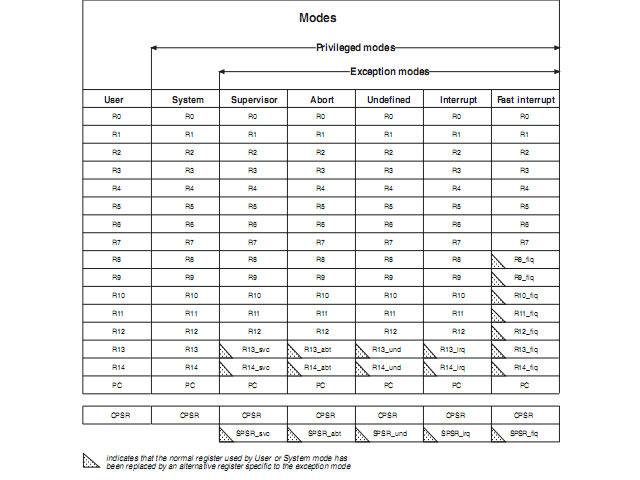
\includegraphics[scale=0.7]{common/register.png}\\
\footnotesize\textbf{Quelle:}\parencite[43]{archManI}
\caption{ARM926EJ-S Register}
\end{figure}
Teilweise sind die Register mehrfach vergeben, denn im ARM Prozessor gibt es unterschiedliche Prozessor-Modi und f\"ur ein gro\ss teil dieser Modi stellt der Prozessor f\"ur R13 und R14 neue Register zur Verf\"ugung. Das spielt dann eine wichtige Rolle wenn man unterschiedliche Stacks f\"ur die Modi aufbauen muss.
\section{Prozessor Modus}
Der ARM926EJ-S stellt sieben unterschiedliche Modi bereit in der sich der Prozessor befinden kann. Jeder dieser Modi kann man per Programmcode betreten oder durch eine Exception. 
\begin{dinglist}{227}
	\item{\textbf{User} \\ Das ist der Modus in dem alle Benutzerprogramme laufen. Sie haben keinen direkten Zugriff auf die Kernel-Routinen, sondern m\"ussen daf\"ur Trap-Instruktionen benutzen.}
	\item{\textbf{FIQ(extra R8-R14) }\\ Dieser Modus wird nur von sehr wenigen Interrupts betreten. Das sind die Interrupts die eine sehr hohe Priorit\"at haben und umgehend von dem Prozessor behandelt werden m\"ussen.}
	\item{\textbf{IRQ(extra R13-R14)}\\ Alle Standard Interrupts wie Tastatureingabe und andere die darauf konfiguriert werden, landen in diesem Modus. Routinen in diesem Modus k\"onnen in den User-Modus wechseln um User-Programme auszuf\"uhren.}
	\item{\textbf{Supervisor(extra R13-R14)} \\ Dieser Modus ist ausschlie\ss lich f\"ur Trap-Routinen reserviert. Das bedeutet alle Instruktionen die von einem Userprogramm aufgerufen wurden um Kernel-Methoden auszuf\"uhren.}
	\item{\textbf{Abort(extra R13-R14)}\\ Abort ist der Modus in den der Prozessor f\"allt wenn entweder eine Instruktion aufgrund eines Fehlers abgebrochen werden muss oder ein Fehler beim Abruf einer Speicherstelle auftritt.}
	\item{\textbf{Undefined(extra R13-R14)}\\ Dieser Modus wird nur dann betreten sofern der ARM-Prozessor eine Instruktion von einem Co-Prozessor anfordert dieser aber nicht reagiert.}
	\item{\textbf{System} \\ Dieser Modus ist nur f\"ur den Kernel und kein User-Programm darf diesen betreten.}
\end{dinglist}
Der System-Mode ist ein spezieller Modus. Dieser wird \"uber keinen Interrupt ausgel\"ost. Er ist deshalb vorhanden weil das Betriebssytem ihn benutzt um Betriebssytem relevante Resourcen zu benutzen. Weiterhin benutzt dieser Modus die gleichen Register wie der User-Modus.

\chapter{Entwurf}
\section{Einleitung}
In den vorherigen Kapiteln wurde gekl\"art welche Anforderungen an \mops gemacht werden. In dem nun folgenden Kapitel wird eine Idee pr\"asentiert wie diese Komponenten miteinander interagieren sollen. Um einen groben \"Uberblick \"uber die Idee zu verschaffen soll dieses Kapitel mit einem Bild eingeleitet werden.
\begin{figure}[h!]
	\centering
	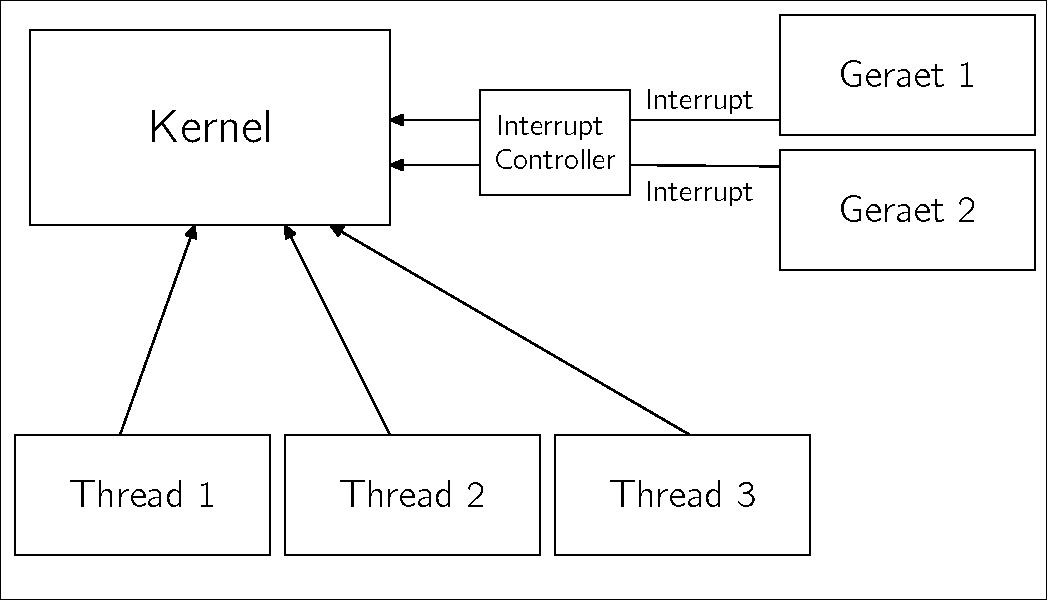
\includegraphics[scale=0.60]{common/draft-overview.pdf}	
	\caption{\mops \"Uberblick}
	\label{draft:overview}
\end{figure}\\
\mops besteht im Gro\ss en und Ganzen aus vier \"ubergeordneten Komponenten. 
\begin{dinglist}{227}
	\item{\textbf{Ger\"ate}} \\ 
	Wie in den Anforderungen beschrieben besteht \mops auf zwei Hardwarekomponenten. Diese Komponenten k\"onnen Interrupts ausl\"osen um mit dem Betriebssystem zu kommunizieren.
	\item{\textbf{Interrupt Controller}} \\
	Damit kommen wir zu einem weitern Punkt der \mops pr\"agt. Der Interrupt-Controller ist, wie in den Anforderungen beschrieben, eine Hardwarekomponente die auf den Chip integriert ist und die Priorisierung und Weiterleitung von Interrupts an das Betriebssystem steuert.
	\item{\textbf{Threads}} \\
	Die Threads stellen unter anderem die User-Programme in dem Betriebssystem dar. Sie k\"onnen mit dem Kernel interagieren und werden von dem Kernel verwaltet.
	\item{\textbf{Kernel}} \\ 
	Der Kernel ist der Hauptbestandteil von \mops, er stellt die Schnittstelle zu s\"amtlicher Hardware und den Threads dar.
\end{dinglist}
\section{Ger\"ate}
Die Ger\"ate stellen neben dem Kernel und den Threads eine sehr wichtige Rolle in \mops dar. Die Ger\"ate k\"onnen \"uber Interrupts mit dem Kernel kommunizieren. Hierbei handelt es sich um eine hardware-basierte Interprozesskommunikation.
\section{Interrupt-Controller}
Wie aus der Abbildung \ref{draft:overview} ersichtlich liegt zwischen den Ger\"aten und Kernel der sogenannte Interrupt-Controller, eine Hardwarekomponente die die Priorisierung und Verwaltung von Interrupts \"ubernimmt. In der Idee von \mops hat der Interrupt-Controller die Funktion die Quellen der Interrupts zu lokalisieren und die passenden Interrupt-Service-Routine bereitzustellen, sodass diese von dem Kernel ausgef\"uhrt werden k\"onnen. Abbildung \ref{draft:draft-vic} soll das verdeutlichen.
\begin{figure}[h!]
	\centering
	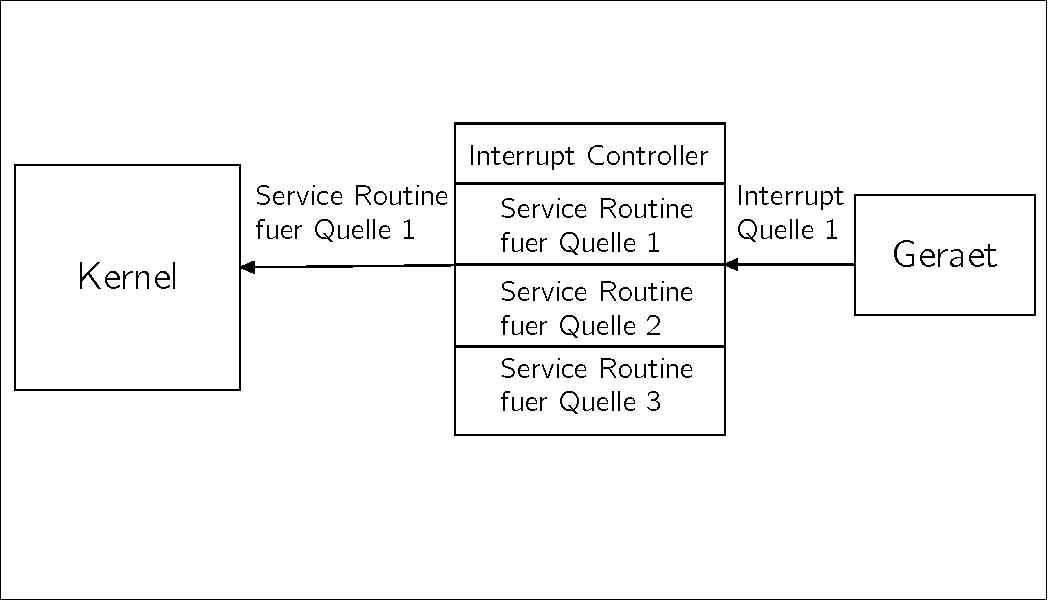
\includegraphics[scale=0.60]{common/draft-vic.pdf}	
	\caption{Interrupt-Controller}
	\label{draft:draft-vic}
\end{figure}
\newpage
\section{Threads}
In den Anforderungen wurde beschrieben das \mops aus drei Threads besteht. Diese Threads stellen User-Programme dar die \"uber bestimmte Routinen mit dem Kernel kommunizieren jedoch aber auch von Interrupts unterbrochen werden k\"onnen. Ein Thread ist in \mops, wie auch in vielen anderen Betriebssystemen, ein Abbild von einem Prozess der definierte Aktionen ausf\"uhrt, z.B. eine Berechnung oder eine Ausgabe. Damit diese Aufgabe nicht der Kernel \"ubernehmen muss existieren eben genannte Threads. Aufgrund der Tatsache das \mops keine Festplatte oder ein anderes dauerhaft beschreibbares Medium besitzt, m\"ussen die Threads alle in den RAM geladen werden. Die Idee von \mops war es also die Threads in einen definierten Bereich im RAM zu laden. Die folgende Abbildung zeigt diesen Sachverhalt.
\begin{figure}[h!]
	\centering
	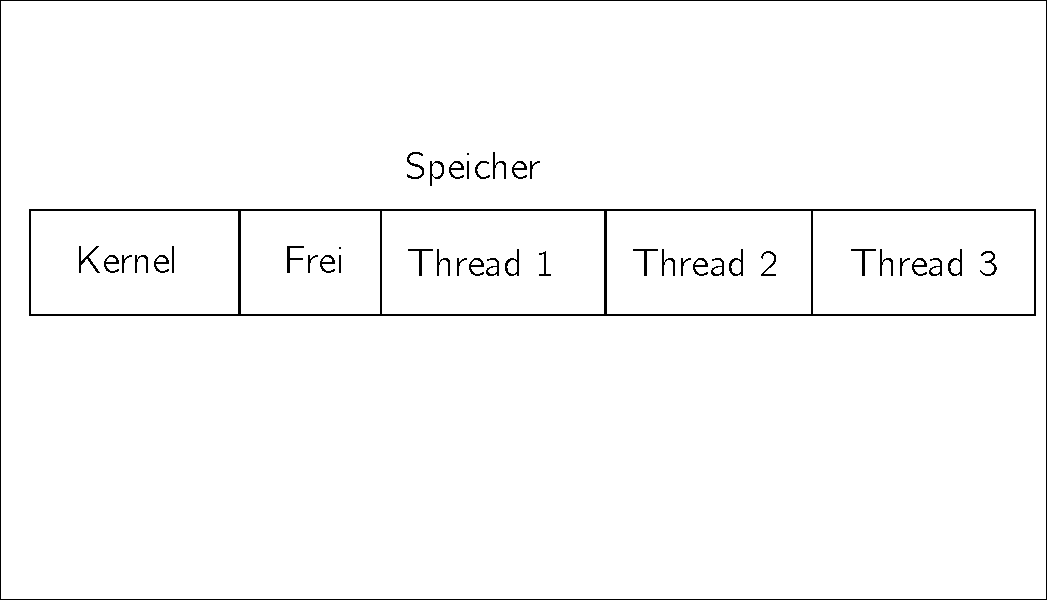
\includegraphics[scale=0.60]{common/draft-thread-overview.pdf}	
	\caption{Thread-Layout im RAM}
	\label{draft:draft-thread-overview}
\end{figure}\\
An erste Stelle liegt nat\"urlich der Kernel, dann kann noch etwas freier Plaz kommen und danach liegen alle Threads hintereiander im RAM.
\\\\
Wie schon in den Anforderungen beschrieben ist es \mops nicht m\"oglich Threads zur Laufzeit zu erzeugen sondern es kann nur die vordefinierten starten und verwalten. Es musste also eine Vorgehensweise entwickelt werden wie diese Threads in den RAM kommen und vor allem, wie sie in \mops integriert werden konnten. \\
Hierzu entstand die Idee der RAM-Disk. Das ist eine Datei in der die Informationen zu den Threads gespeichert wurden. Nun stellt sich nat\"urlich die Frage welche Informationen das sind. Die Frage l\"asst sich ganz einfach beantworten: \textbf{Die Information die einen Thread klassifizieren muss ohne Zweifel der Assembler-Code des Threads}. 
\newpage
\begin{figure}[h!]
	\centering
	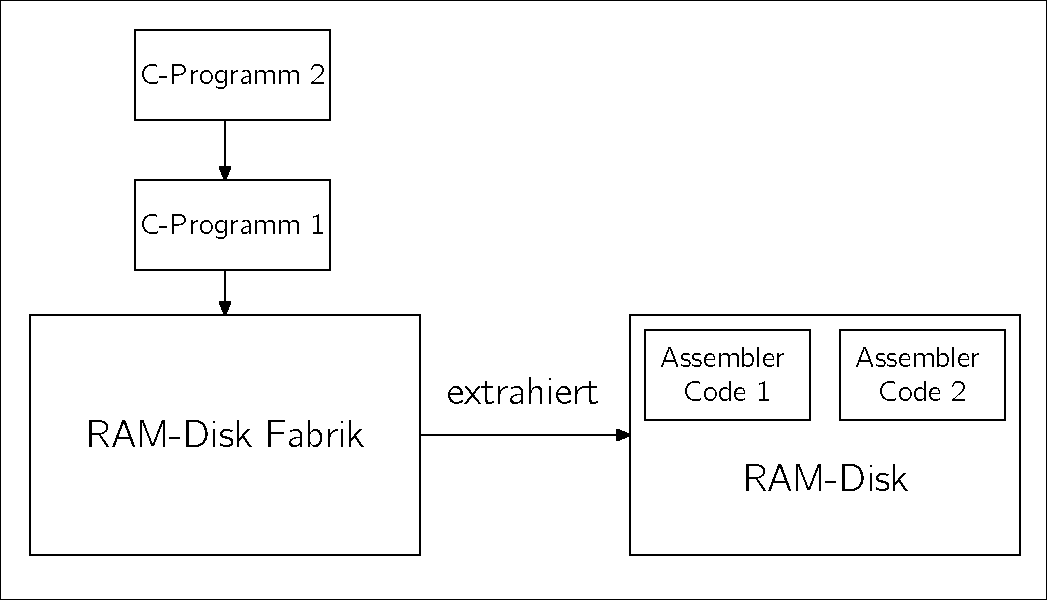
\includegraphics[scale=0.60]{common/draft-thread-ramdisk.pdf}	
	\caption{Erstellung der RAM-Disk}
	\label{draft:draft-thread-ramdisk}
\end{figure}
\noindent
Die Idee die in \mops verfolgt wurde bestand darin einfache C-Programme zu entwerfen und diese durch ein Programm zu schicken das den Assembler-Code dieser Programme extrahiert. In Abbildung \ref{draft:draft-thread-ramdisk} ist zu erkennen das zwei Programme durch die sogenannte RAM-Disk Fabrik wandern und diese extrahiert den Assembler-Code und verpackt ihn in die daf\"ur vorgesehene RAM-Disk. Der entstandene Assembler-Code kann dann von einem \mops -definierten Lader in den Speicher bef\"ordert werden.\\\\
Neben dem vorbereiten und Laden der Threads in den RAM ist es aber auch notwendig die Threads zu verwalten. Diese Aufgabe \"uebernimmt unter anderem der Kernel.
\section{Kernel}
Der Kernel ist der Teil von \mops der s\"amtliche Verwaltungsaufgaben \"ubernimmt die man sich vorstellen kann. Das geht von den Interrupts bis hin zur Verwaltung der Threads.
\begin{figure}[h!]
	\centering
	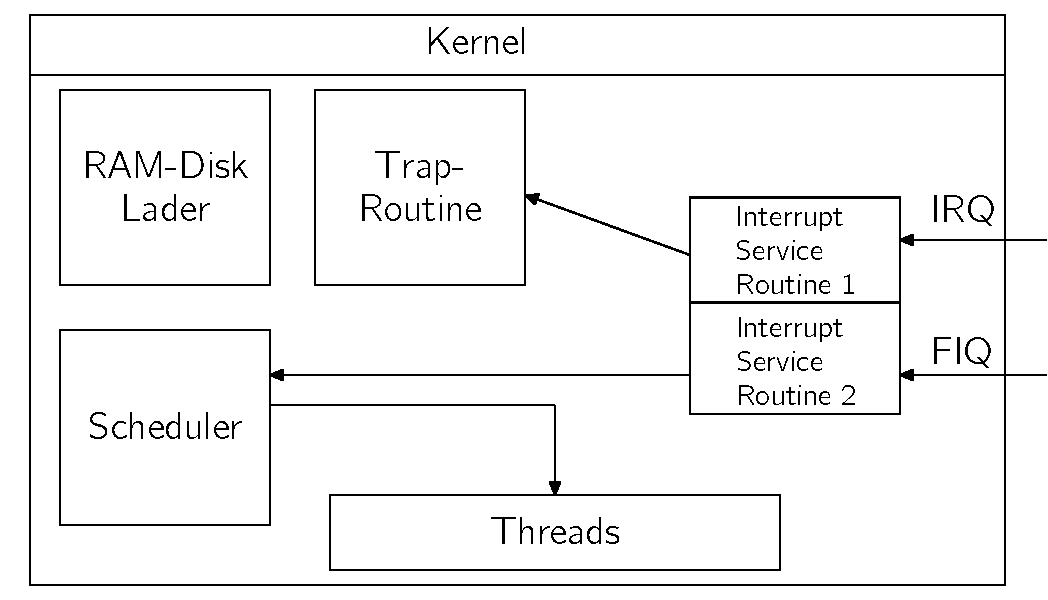
\includegraphics[scale=0.60]{common/draft-kernel.pdf}	
	\caption{Kernel - \"Uberblick}
	\label{draft:draft-kernel}
\end{figure}\newpage\noindent
Die Abbildung \ref{draft:draft-kernel} gibt nochmal eine detailierten Einblick in das Innenleben des Kernels. Zu sehen sind hier alle Komponenten die auf die Idee mit Einfluss hatten. Der RAM-Disk Lader, Interrupt-Service Routinen, der Scheduler und die Trap-Routinen. Diese Abbildung soll darstellen wie ein normaler Ablauf in dem Kernel aussehen kann. \\
Im ersten Schritt kommt ein Interrupt oder Fast-Interrupt-Request in das System, der Interrupt-Controller priorisiert diesen dann und stellt dem Kernel die passende Interrupt-Service Routine zur Verf\"ugung. Die jeweilige Routine kann dann z.B. entweder einen Trap-Routine Aufrufen oder aber, was wesentlich interessanter ist, den Scheduler. Dieser Scheduler geht dann an die Thread-Tabelle und greift sich einen neuen Thread der jetzt in den Prozessor geladen wird. Womit wir beim n\"achsten Punkt sind.\\ \\
Der Scheduler ist ein Manager f\"ur die Verwaltung der Prozessorzeiten und Priorisierung der Threads.
\begin{figure}[h!]
	\centering
	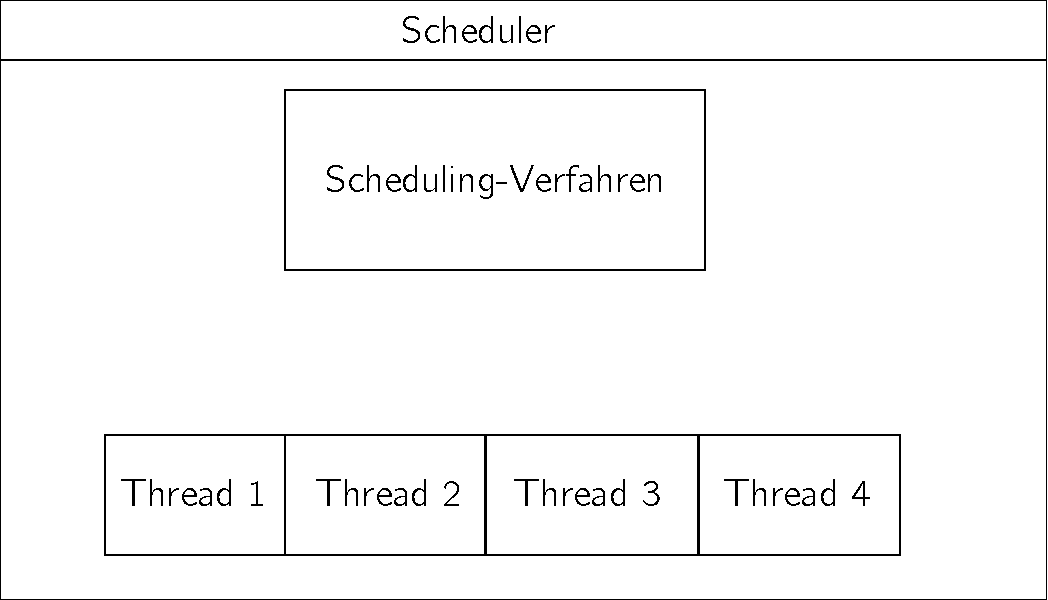
\includegraphics[scale=0.60]{common/draft-scheduler.pdf}	
	\caption{Scheduler}
	\label{draft:draft-scheduler}
\end{figure}\\
Er setzt sich aus zwei wichtigne Komponenten zusammen. Dem Scheduling-Verfahren, welches frei gew\"ahlt werden kann und einer Tabelle von Threads. Aus dieser Tabelle w\"ahlt der Scheduler, je nach Scheduling-Verfahren, einen Thread aus und \"ubergibt ihm die Kontrolle. Es gibt viele Scheduling-Verfahren, aber hier wurde sich jedoch einer Idee bedient die in der fr\"uhzeitigen Entwicklung von Schedulern weit verbreitet war. 
\newpage\noindent
Das Verfahren nennt sich \textbf{Round-Robin-Verfahren}. Die folgende Grafik soll das Verfahren beschreiben.
\begin{figure}[h!]
	\centering
	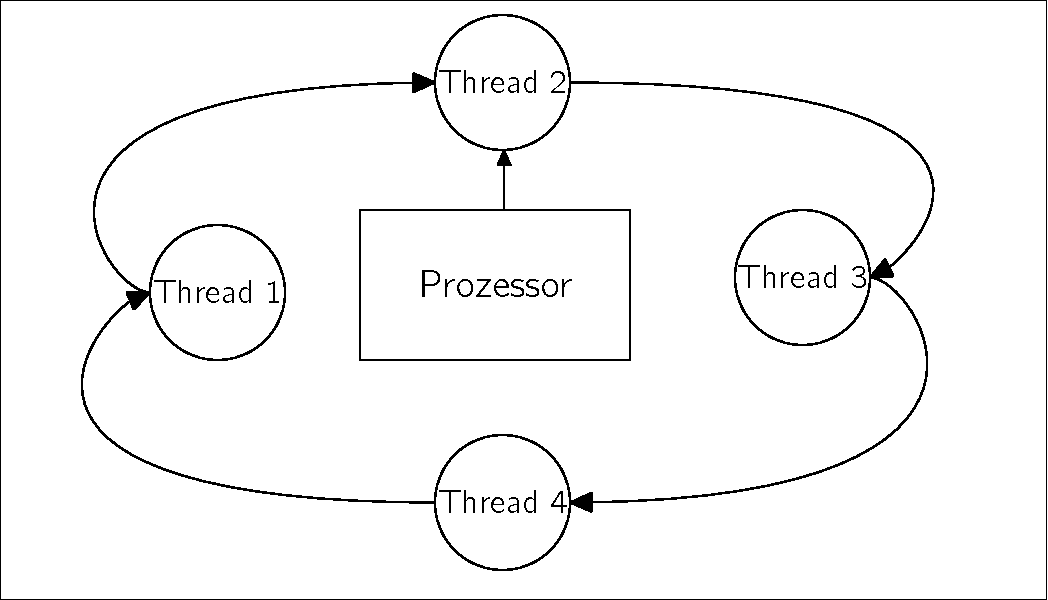
\includegraphics[scale=0.60]{common/draft-roundrobin.pdf}	
	\caption{Round-Robin Verfahren - Schematisch}
	\label{draft:draft-roundrobin}
\end{figure}\\
Beim Round-Robin Verfahren wird der Scheduler so entwurfen das er jedem Thread eine fixe Zeitspanne an Prozessorzeit zusichert und die Kontrolle dann an den jeweiligen Thread \"ubergibt. Nach Ablauf der Zeit wird dann der n\"achsten Thread in der Tabelle aufgerufen. Diese Verfahren wurde f\"ur \mops deshalb gew\"ahlt weil in Handheld Ger\"aten keine Sonderpriorisierungen stattfinden m\"ussen und die Umsetzung in den Zeitrahmen passte.
\chapter{Konkretisierung des Entwurf}
\section{Einleitung}
Die Entwicklung von \mops erfolgte in mehreren Schritten. Wichtige Zwischenstopps waren hier der Startprozess, die Exceptionhandler, der Interrupt-Controller, die Interrupt-Serviceroutinen und das Threadmanangment. Jeder dieser Punkte bedurfte ein einzelne Entwurfsphase auf die jetzt genauer eingegangen werden.
\section{Startmechanismus}
\label{e1:start}
Der Startprozess unterteilt sich in drei Schritte:

	\begin{figure}[h]
		\centering
					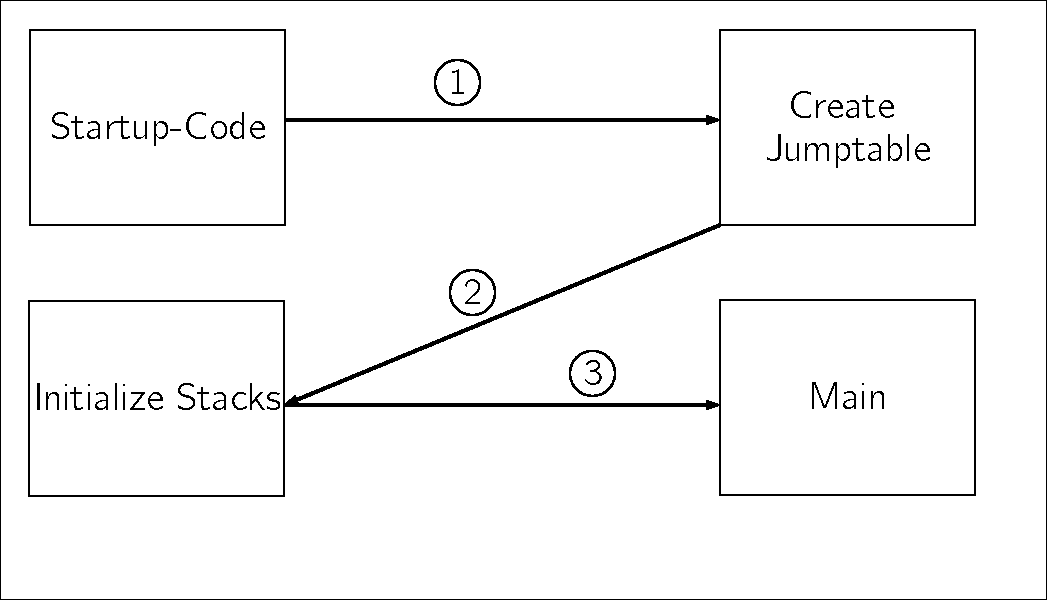
\includegraphics[scale=0.60]{common/kernel-img.pdf}	
		\caption{Kernel-Image Version 1}
		\label{draft:kernelImage}
	\end{figure}
	\begin{enumerate}
		\item{\textbf{Startup-Code}}\\
		 Der Emulator springt an die Adresse \texttt{0x000000}\footnote{\textit{Diese Adresse wird \"uber das Linker-Script bestimmt}}, an dieser Stelle steht die erste Assemblerroutine des Betriebssystems. Diese Routine dient dazu um gewisse Vorbedingungen zu erstellen. Eine davon ist die nachfolgende.
		 \item{\textbf{Interrupt Handler}}\\
		 \label{draft:exceptionHandler}
Interrupts k\"onnen von externen oder internen Ressourcen ausgel\"ost werden. Damit der Prozessor wei{\ss} wo er im Falle eines Interrupts hinspringen muss, schreibt ARM eine Struktur vor die eingehalten werden muss \parencite[vgl.][54]{archManI}. 
			\begin{figure}[h]
				\centering
					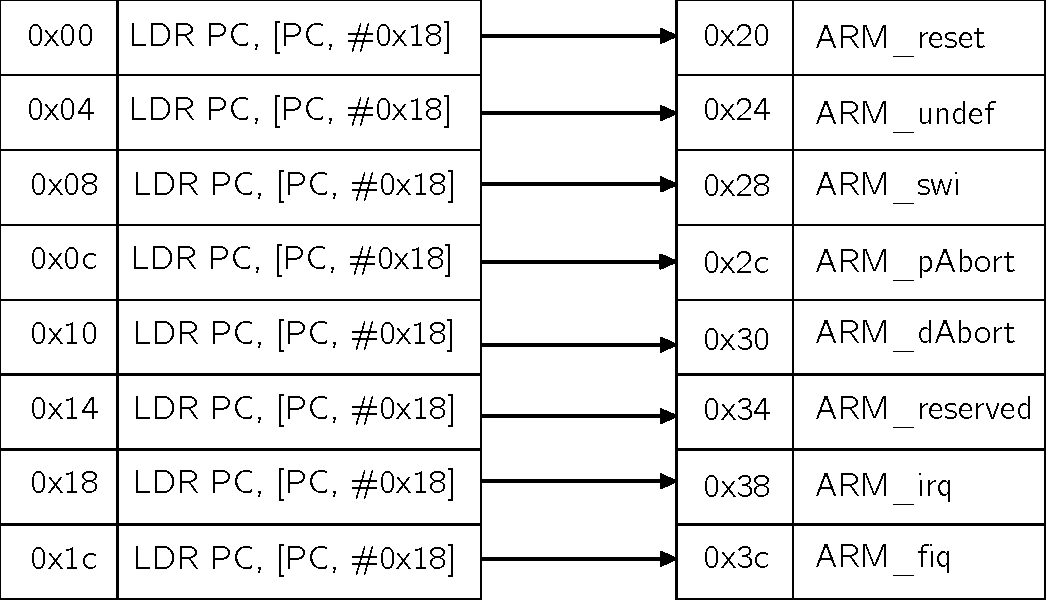
\includegraphics[scale=0.6]{common/exceptionhandler.pdf}
				\caption{Erzeugen der Sprungtabelle}
				\label{draft:excptionTable}
			\end{figure}\\
			In diesem Schritt ist erkennbar, dass es zwei Tabelle gibt die von dem Programmierer erstellt werden m\"ussen. Die erste Tabelle enth\"alt Programm-Relative Adressen auf eine zweite Tabelle. In der zweiten Tabelle befinden sich dann die konkreten Adressen der Exceptionhandler. Neben der Exception f\"ur einen Reset des Systems gibt es noch weitere Exceptions wie die Undefined Operation (ARM\_undef), Softwareinterrupt (ARM\_swi), Prefetch-Abort (ARM\_pAbort), Data-Abort(ARM\_dAbort),  die Reserved Exception (ARM\_reserved) und ganz wichtig zu erw\"ahnen der IRQ (ARM\_irq und FIQ (ARM\_fiq).\\\\
Der Vorteil des Mechanismus, Programmrelative Adresse anstatt die direkten Handler zu laden, besteht darin das man so leicht die Handler austauschen oder zus\"atzliche hinzuf\"ugen kann ohne dabei den Assemblercode zu \"andern.\\
Neben der Erstellung der Sprungtabelle f\"ur die Exceptionhandler, ist es weiterhin notwendig den Stack f\"ur die jeweiligen Prozessormodi zu definieren, dies geschieht im n\"achsten Schritt.
		\item{\textbf{Erstellung der Stacks mit anschlie\ss enden Sprung in main}}\\
		\label{draft:stack}
		Die f\"ur \mops relevanten Modi des Prozessors sind 
		\begin{dinglist}{227}
			\item{IRQ-Modus}
			\item{FIQ-Modus}
			\item{System-Modus}
			\item{Supervisor-Modus}
		\end{dinglist}
		Jeder dieser vier Modi, bis auf den System-Modus, hat seinen eigenen Stackpointer und f\"ur jeden muss dementsprechend der passende Stackpointer gesetzt werden. Das ist deshalb notwendig da im Falle einer Exception der Prozessor in den jeweiligen Modus wechselt und wenn kein valider Stackpointer vorhanden ist kann es zu undefinierten Verhalten kommen. Die Gr\"o\ss e der Stackpointer l\"asst sich \"uber das Link-File bestimmen, f\"ur \mops wurde eine Gr\"o\ss e von 8KB je Modus gew\"ahlt.\\
Sobald die Stacks alle initialisiert sind erfolgt der Sprung in die \texttt{main} Routine des Betriebssystem. Ab hier finden nun weitere Schritte statt um das System fertig zu initialisieren.
	\end{enumerate}
\section{Interrupt-Controller}
Ein Interrupt-Controller stellt in einem Betriebssystem die Schnittstelle zwischen den Interrupts und der Hardware dar Er priorisiert die Interrupts, die von externen wie auch internen Quellen ausgel\"ost werden k\"onnen, und leitet sie an das Betriebssystem weiter. Es gibt zwei Arten von Controllern:
\begin{dinglist}{227}
	\item{Non-Vectored Interrupt-Controller}
	\item{Vectored Interrupt-Controller}
\end{dinglist}
Die erste Version, \textbf{Non-Vectored Interrupt-Controller}, stellt nur die M\"oglichkeit bereit einen Interrupt abzufangen, jedoch muss sich der Programmierer darum k\"ummern welche Quelle den Interrupt ausgel\"ost hat, die Priorit\"at ermitteln und die passende Interrupt-Service Routine herausfinden. Das klingt zwar im ersten Moment ganz logisch und sinnvoll, ist aber mit einer Menge Code verbunden und stellt deshalb eine sehr gro\ss e Fehlerquelle dar.\\
Der Vectored Interrupt-Controller ist eine in Hardware gegossene Komponente auf dem Board welches man benutzt. Er bietet die Konfigurationsm\"oglichkeit zu definieren, welche Interrupts von welchen Quellen ausgel\"ost werden k\"onnen, welche Priorit\"aten sie haben und welche Interrupt-Service Routinen f\"ur diese Interrupts zur Verf\"ugung gestellt werden. Nun brauch man im Falle eines Interrupts keine umfangreichen Mechanismen lostreten um die Quellen zu ermitteln, sondern der Interrupt-Controller stellt jetzt alle diese Informationen bereit. Die Installations dieses Controllers ist zwar komplexer als die der ersten Version, aber die M\"oglichkeiten sind breiter und die Benutzung ist komfortabler. Aus diesen Gr\"unden wurde sich bei \mops f\"ur den \textbf{Vectored Interrupt Controller} entschieden.
Das folgende Bild ist eine schematische Darstellung des Vectored Interrupt-Controller.

\begin{figure}[H]
	\begin{center}	
	\caption{Vectored Interrupt Controller}
	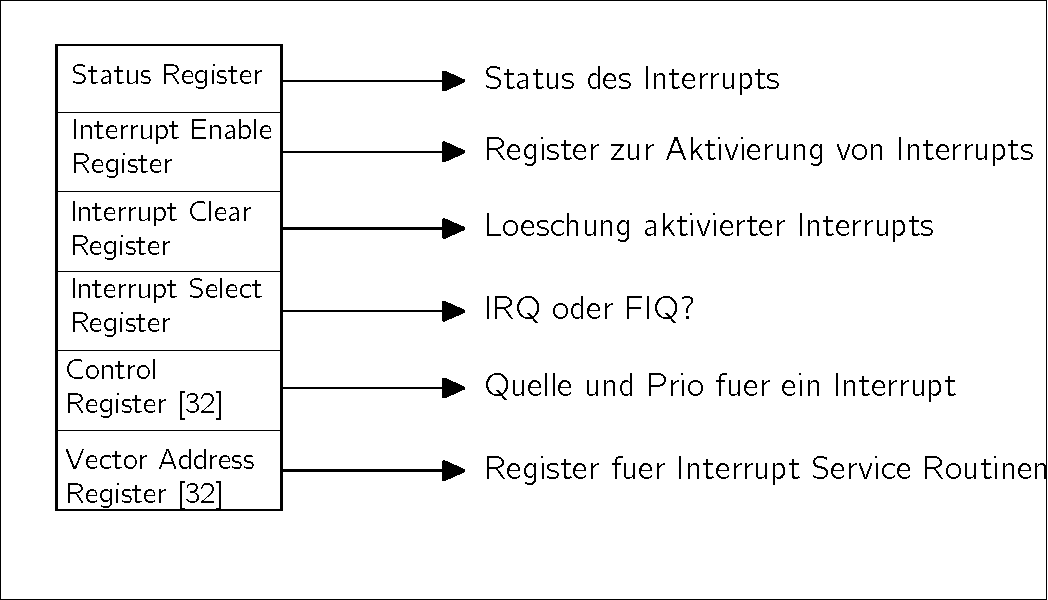
\includegraphics[scale=0.60]{common/vic.pdf}
	\end{center}
	\label{vicSchema}
\end{figure}
\noindent
Sofern das Board einen Vectored Interrupt-Controller zur Verf\"ugung stellt ist dieser an einer bestimmten Adresse lokalisiert. Bei dem von \mops emulierten System ist die Adresse \texttt{0x10140000}\parencite[vgl.][223]{archManI}. Ab dieser Adresse beginnt der Adressbereich des Controllers, hier befinden sich oben genannte Register wie Statusregister, Interrupt Enable Register, Interrupt Clear Register, Interrupt Select Register etc., desweiteren sind hier auch die f\"ur die Interrupt Vectoren wie auch die Control Register f\"ur die jeweiligen Interrupts \parencite[vgl.][35]{vic}.\\\\
Die relevanten Register f\"ur \mops sind die Vector Address Register, Control Register, Interrupt Enable, Interrupt Clear und Interrupt Select Register. \"Uber diese ist es m\"oglich die Service Routinen f\"ur die Interrupts zu definieren, wie auch die Priorit\"aten und ob der konfigurierte Interrupt als ein IRQ oder FIQ behandelt werden soll. Mit der folgenden Grafik wird schematisch dargestellt wie eine Konfiguration des Controllers aussehen kann.
\begin{figure}[H]
	\begin{center}	
	\caption{Konfigurationsbeispiel VIC}
	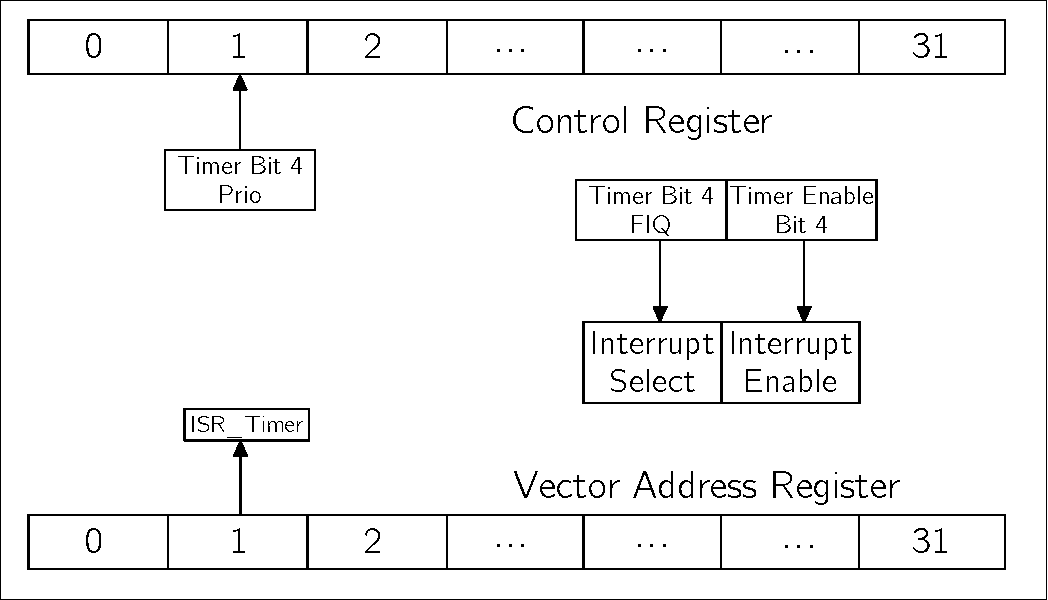
\includegraphics[scale=0.60]{common/vicsample.pdf}
	\end{center}
	\label{draft:vicSample}
\end{figure}
\noindent
Dieses Beispiel zeigt eine Beispielkonfiguration des Timerinterrupts. Um diesen Interrupt zu konfigurieren sind vier Schritte notwendig:
\begin{dinglist}{227}
	\item{Installation der Adresse der Interrupt Service Routine}
	\item{Konfiguration des Control Register mit Priorit\"at des Timers}
	\item{Entscheidung ob der Interrupt als IRQ oder FIQ ausgel\"ost werden soll}
	\item{Aktivierung der Interrupt-Ausl\"osung}
\end{dinglist}
F\"ur den \textit{Timer0-Interrupt} muss an dieser Stelle das 4. Bit \parencite[vgl. Tabelle 4-40][227]{archManI} in dem Interrupt-Controller setzen. Das gilt sowohl f\"ur die Aktivierung, Auswahl des Interrupts als auch die Priorit\"at.

\section{Interrupt-Service Routinen}
Nachdem die Interrupts konfiguriert wurden ist es notwendig die Interrupt-Service Routinen der Interrupts zu definieren. Beispielhaft werden hier die Routinen des Timers und des UART0-Interrupts pr\"asentiert.
\begin{figure}[H]
	\begin{center}	
	\caption{Interrupt Service-Routinen Timer \& UART0}
	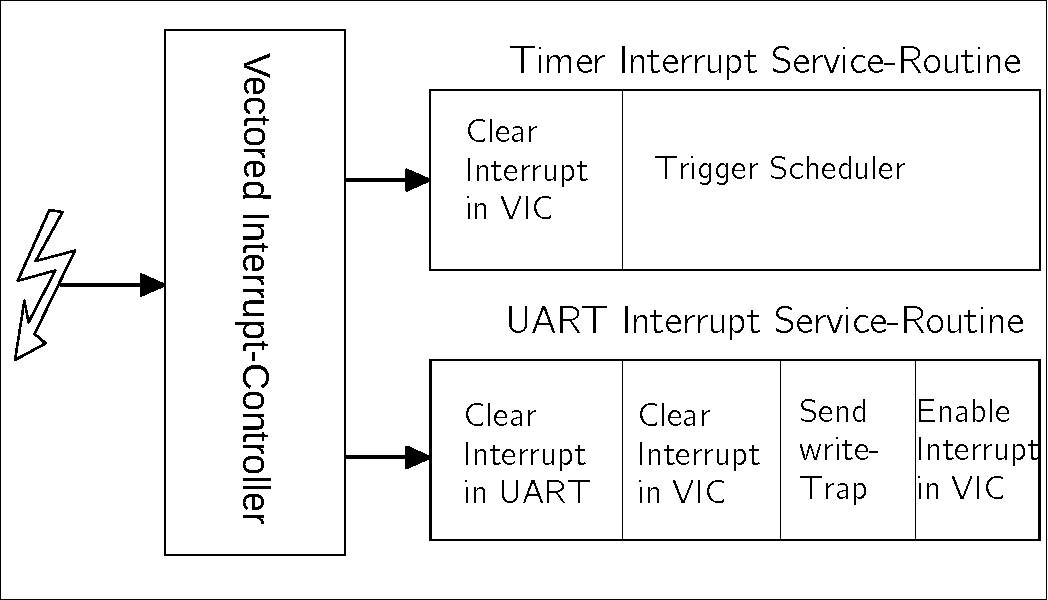
\includegraphics[scale=0.60]{common/isr.pdf}
	\end{center}
\end{figure}
\noindent
Sobald der Interrupt ausgel\"ost wurde behandelt der Controller diesen und leitet es an die zugeh\"orige Routine zur Behandlung weiter. Im Beispiel des Timers, wird hier der Interrupt erst im Controller auf 'Behandelt' gesetzt und dann wird der Scheduler aufgerufen um dem n\"achsten Prozess zu starten. Das L\"oschen des Interrupts im Controller ist deshalb erforderlich, damit ein neuer Interrupt ausgel\"ost werden kann, denn nur nachdem der Interrupt als behandelt markiert wurde, kann ein neuer erzeugt werden. \\ In der aktuellem Implementation von \mops gibt es zwei Interrupts auf die reagiert wird. Zum einen ist das der \textit{Timer0}-Interrupt und zum anderen der Interrupt des \textit{UART0}-Interface. Bei Bedarf kann man auch noch weiter Interrupts definieren, dazu muss jedoch die Konfiguration des VIC abg\"andert werden.
\newpage
\section{Syscalls}
Neben den IRQ und FIQ spielen die Syscall auch noch eine sehr wichtige Rolle. Im Rahmen der ARM-Architektur wurden die Syscalls mit dem Namen \textit{Software Interrupts} bezeichnet. Sicherlich ist der Name Syscalls oder Traps gel\"aufiger. Um aber konsitent zu bleiben, wird im laufenden der Name Software Interrupt(SWI) verwendet.\\
Ein SWI ist ein Interrupt der nicht im Kernel-Modus l\"auft aber Kernel-Routinen aufrufen darf. Das ist dann sinnvoll, wenn ein User-Programm Zugriff auf eine Kernel-Routine (wie das Schreiben auf die Konsole) ben\"otigt. Wie in Abbildung \ref{draft:excptionTable} zu erkennen ist, wird bei einem SWI-Interrupt die ARM\_swi Routine angsprungen. Diese Routine leitet den Interrupt-Request an eine weitere Komponente weiter die schematisch wie folgt aussieht.
\begin{figure}[H]
	\begin{center}	
	\caption{SWI-Handler}
	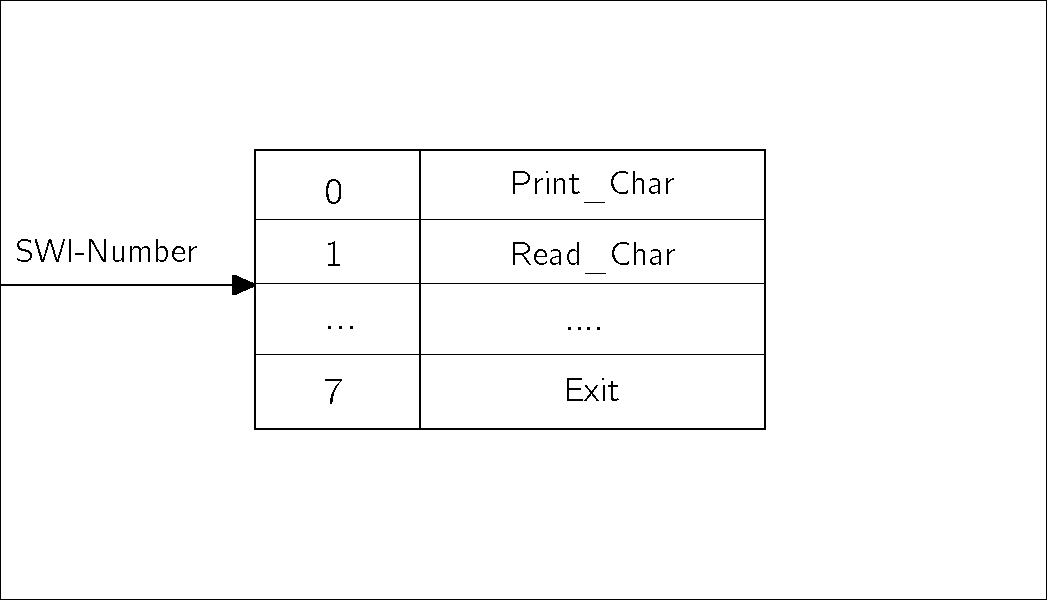
\includegraphics[scale=0.60]{common/swihandler.pdf}
	\end{center}
\end{figure}
\noindent
In der aktuellen Fassung von \mops ist nur der SWI-Handler f\"ur den \texttt{Print\_Char}-SWI definiert, es sollen jedoch weitere folgen.
\section{Threadmanagment}
\subsection{Threadlayout}
Das Threadmanagment spielt eine wichtige Rolle in jedem Betriebssystem. Aufgrund der Komplexit\"at und des zeitlichen Faktors wurde bei \mops auf ein rudiment\"areres System gesetzt. Das bedeutet das keine Threads zur Laufzeit des Systems geladen werden k\"onnen sondern die Threads vor Beginn definiert werden mussten.\\
Eine abstrakte Darstellung dieses Thread-Image kann man sich wie folgt vorstellen:
\begin{figure}[H]
	\begin{center}	
	\caption{Thread-Image}
	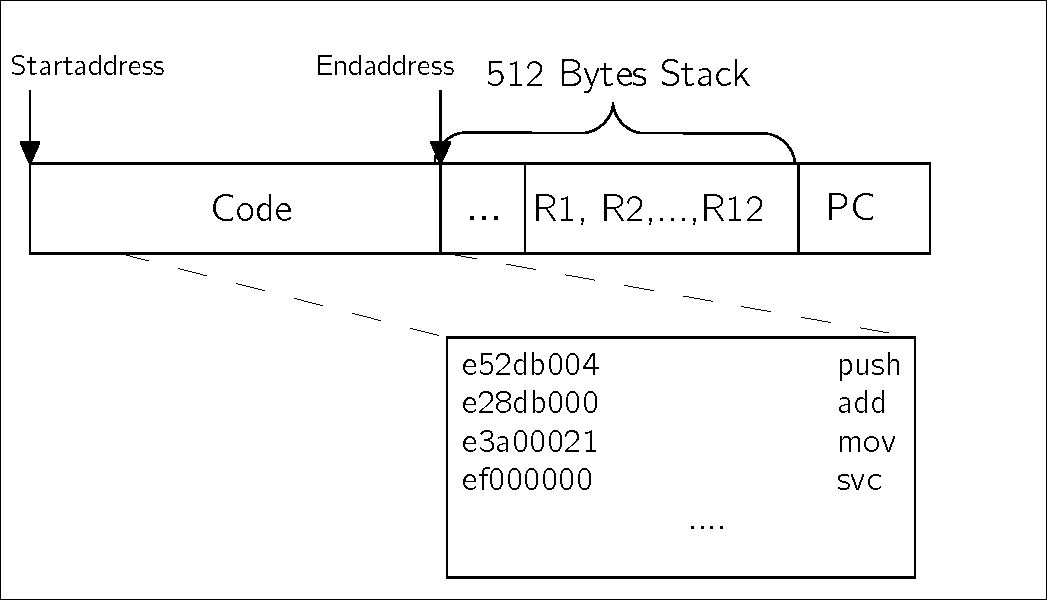
\includegraphics[scale=0.60]{common/threadimage.pdf}
	\end{center}
\end{figure}
\noindent
Diese Struktur wird zu Begin des Betriebssystem im RAM hergestellt. Zuvor muss jedoch doch der Assemblercode aus dem zu ladenen Thread extrahiert werden. Die Threads werden als einfache C-Programme dargestellt. Diese C-Programme werden so rudiment\"ar wir m\"oglich Kompiliert und gelinkt, das bedeutet das s\"amtliche Standardbibliotheken nicht mit gelinkt werden und keine main-Funktion bereitgestellt wird. Die entstandene .ELF-Datei wird dann ins Bin\"arformat umkopiert und danach extrahiert ein Programm den Assemblercode aus der Bin\"ardatei und schreibt diese in eine RAM-Disk. F\"ur \mops wurde eine sehr proprit\"are RAM-Disk gew\"ahlt. Folgende Grafik zeigt eine schematische Darstellung dieser RAM-Disk. 
\begin{figure}[H]
	\begin{center}	
	\caption{RAM-Disk}
	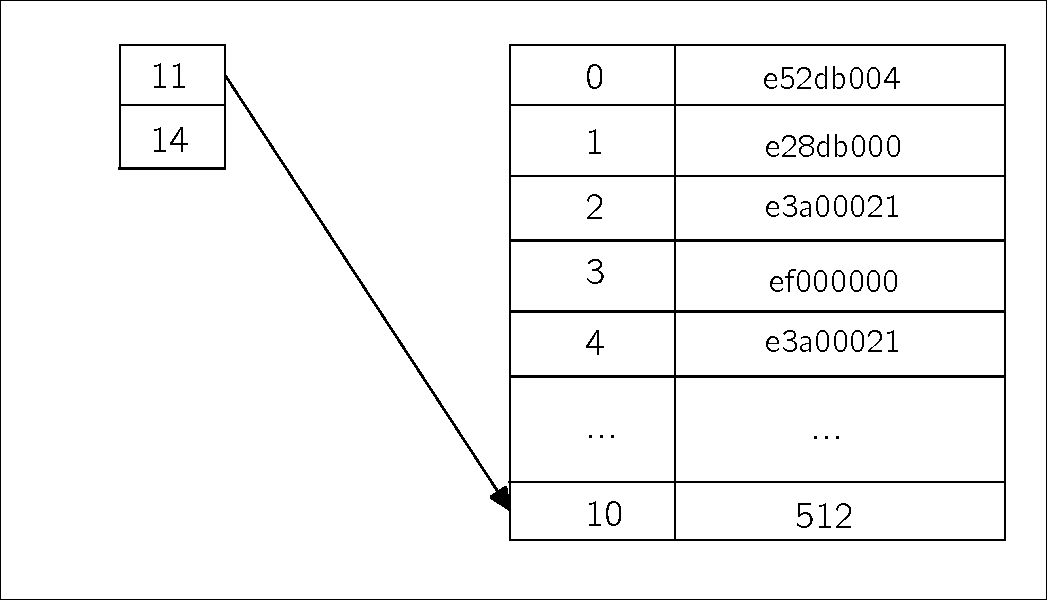
\includegraphics[scale=0.60]{common/ramdisk.pdf}
	\label{ramdisk}
	\end{center}
\end{figure}
\noindent
Nachdem diese RAM-Disk erstellt wurde, kann \mops diese im Betrieb laden und den Assemblercode an die passende Position im RAM laden. Neben den Informationen \"uber den Assembler-Code enth\"alt die RAM-Disk unter anderem die Information wieviel Bytes an Stack f\"ur den Prozess reserviert werden. Dieser Bereich wird dann beim kopieren vorerst nur mit Nullen aufgef\"ullt. \\
Um die M\"oglichkeit offen zu halten mehr als einen Prozess in den RAM zu laden, stellt die RAM-Disk eine weitere Tabelle zur Verf\"ugung in welcher die Informationen zur L\"ange jeder einzelnen Threads eingetragen sind. F\"ur Abbildung \ref{ramdisk} bedeutet dass, das der erste Thread eine L\"ange von 11 aufweist und ab dem 12. Eintrag der n\"achste Thread beginnt.
\subsection{Scheduling}
Sobald der Thread in den RAM geladen wurde, kann das Betriebssytem jetzt den ersten dieser Prozesse starten. Dieser Start manifestiert sich dadurch das der Stackpointer, vom Kernel auf den Start-Bereich des neuen Stacks von dem Thread, umgemappt werden muss. Danach werden alle Register auf dem neuen Stack gesichert und es erfolgt ein Sprung in die Routine die zuletzt aus der RAM-Disk geladen wurde. 
\begin{figure}[H]
	\begin{center}	
	\caption{RAM-Disk}
	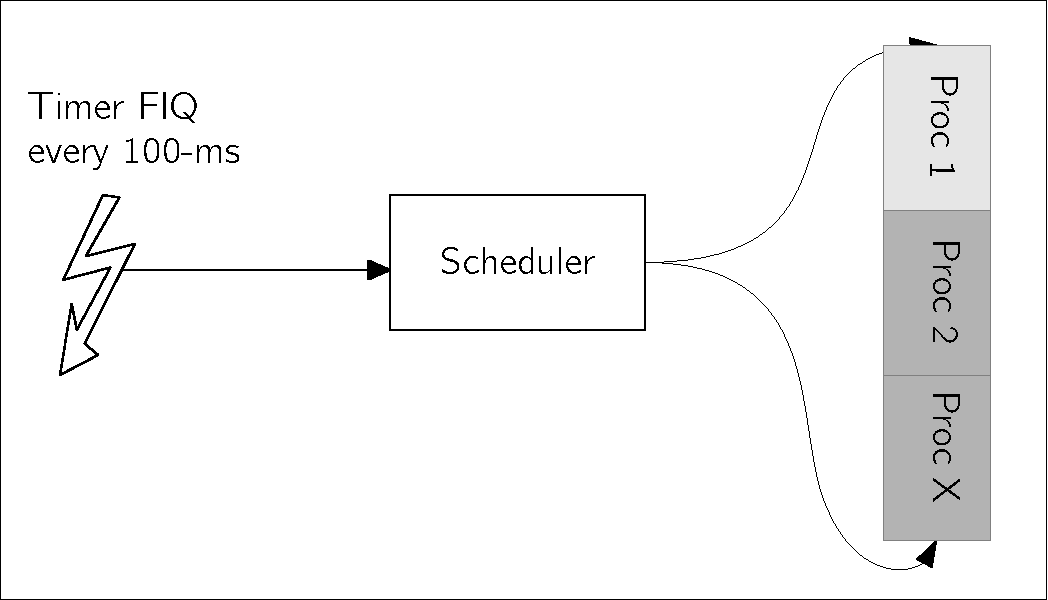
\includegraphics[scale=0.60]{common/scheduler.pdf}
	\label{scheduler}
	\end{center}
\end{figure}
\noindent
In Grafik \ref{scheduler} wird veranschaulicht wie der Mechanismus des Thread-Umschalten in \mops umgesetzt wurde. Hier sieht man das aller 100ms der Timer-Interrupt ausgel\"ost wird und dieser startet den Scheduler. Der Scheduler sucht dann den n\"achsten wartenden Prozess, hier Gelb, raus und schaltet diesen ein. Der andere, momentan gr\"une, wird dann in den wartenden Status geschalten.
Es gibt einige bekannte Scheduling-Verfahren in modernen Betriebssystemen, viele dieser Verfahren kooperieren auch unter bestimmten Umst\"anden um die beste Performance herauszuholen. Hier sind ein paar der wichtigsten Verfahren etwas n\"aher beschrieben:
\begin{dinglist}{227}
	\item{\textbf{First-Come First-Serve}} \\
	Dieses System kann man sich wie eine Schlange an der Post vorstellen. Prozesse werden in eine Queue\footnote{Eine weitverbreitete Datenstruktur in modernen Programmiersprachen die nach dem \textit{First-In First-Out} Prinzip funktioniert.} gepackt und von dort bearbeitet. Dieses System hat jedoch den Nachteil das lange Wartezeiten, durch Prozesse die die CPU sehr \"uberdurschnittlich lange in Anspruch nehmen, entstehen k\"onnen.
	\item{\textbf{Shortest-Job-First}}\\
	W\"ahrend bei diesem Verfahren darauf abgezielt wird den Prozessen die CPU-Zeit zu \"uberlassen welche am k\"urzesten sind. Wie in \cite[189]{scheduling} geschrieben 
\begin{quote}
	\textquote{\textit{This  algorithm associates with each process  the length of the 
process's next CPU burst.}}
\end{quote}
versucht dieser Algorhithmus anhand der CPU-Bursts\parencite[vgl.][184]{scheduling} zu ermitteln wie lange ein Prozess in etwa ben\"otigen wird. Anhand dieser Informationen wird also dann der n\"achste Prozess ermittelt der an der Reihe ist.
Sollten jedoch zwei Prozesse die gleichen CPU-Bursts haben, so wird das \textit{First-Come First-Serve} Verfahren angewendet. Der Vorteil hier ist nat\"urlich das es wesentlich optimaler als die vorherig genannten, jedoch ist es auch komplizierter zu implementieren.\\
	\item{\textbf{Round-Robin}}\\
	Dieses Verfahren 
		\textquote{\textit{is designed especially for  time-
sharing systems.}}\parencite[vgl.][194]{scheduling}
Das bedeutet das der Algorhitmus eine kleine Zeitscheibe definiert in der der Prozess die CPU bekommt. Danach werden die Prozesse die sich in der ``Ready-Queue'' befinden abgearbeitet und jeder bekommt f\"ur die vorher bestimmte Zeit die CPU. Diese Queue wird als eine Ring-Liste behandelt, das hat den Effekt das der Scheduler immer wieder jeden Prozess kurz rannimmt. Der Vorteil dieses Mechanismus ist das jeder Prozess gleich bewertet wird und das es relativ einfach zu implementieren ist. Jedoch bringt genau dieser Vorteil auch einen Nachteil mit sich, n\"amlich das Prozesse die eigentlich eine l\"angere Zeitschreibe br\"auchten immer warten m\"ussen bis sie wieder am Zug sind und das kann nat\"urlich zu sehr hohen Latenzen in der Ausf\"uhrung kommen.
\end{dinglist}
Es wurden jetzt eine Reihe von Scheduling-Mechanismen vorgestellt und es musste eine Entscheidung f\"ur \mops getroffen werden. Aufgrund der einfachen Implementation, fiel die Wahl auf das \textbf{Round-Robin} Verfahren. Die Nachteile konnten f\"ur die erste Version von \mops vernachl\"assigt werden.

\chapter{Implementation}
\section{Einleitung}
Bei der Entwicklung von \mops mussten einige wichtige Entscheidung bez\"uglich der Entwicklungs- wie auch Emulationsumgebung getroffen werden. Im folgenden werden diese Entscheidungen von allen Gesichtspunkten beleuchtet. Neben diesen Aspekten gibt es in diesem Kapitel einen tiefen Einblick in die Implementation von \mops. 

\section{Entwicklungsumgebung}
Mit der Entscheidung ein Mini-Betriebssystem zu programmieren stellt sich nat\"urlich auch die Frage mit welchen Werkzeugen man den Code entwickelt. Zur Entwicklung von ARM-basierten Code kann die Entwicklungsumgebung Eclipse\footnote{\url{http://www.eclipse.org/}}  genutzt werden. Dennoch wurde sich f\"ur den konservativen Weg entschieden und die Entwicklung l\"auft seit her mit dem Linux-integrierten Editor \textit{vim}. Die Vorteile gegen\"uber einer Integrierten Entwicklungsumgebung sind die folgenden: \\\\
\textbf{Vorteile:}
\begin{dinglist}{227}
	\item{\textbf{Schnelligkeit}}\\
	 Es ist keine seperate Installation einer IDE notwendig, denn \textit{vim} ist auf jedem Linux System vorinstalliert. Weiterhin startet \textit{vim} in einer sehr kurzen Zeit.
	\item{\textbf{Unabh\"angigkeit}}\\
	Sollte die Entwicklung auf einem anderen System weitergehen, so ist es nicht notwendig IDE abh\"angige Einstellungen vorzunehmen.
	\item{\textbf{Kontrolle}}\\
	Viele IDEs bringen ein umfangreiches Portfolio an Funktionen mit sich, die jedoch auch Problematisch werden k\"onnen wenn nicht mehr klar ist was f\"ur Schritte die IDE neben den eigentlich notwendigen noch durchf\"uhrt. Da \textit{vim} ein rein textbasierter Editor ist, kann man hier sicher sein das keine unklaren Sachen im Hintergrund passieren.
\end{dinglist}
Jedoch bringt die Entwicklung ohne IDE auch Nachteile mit sich, die hier nicht au\ss en vorgelassen werden d\"urfen.\\ \\
\textbf{Nachteile:}
\begin{dinglist}{227}
	\item{\textbf{Komplex}}\\
	\textit{vim} ist kein Werkzeug f\"ur Anf\"anger, da es sehr nativ und durchaus eine gewisse Zeit bedarf die Verwendung gut zu beherrschen, hier sind die IDEs teilweise klar im Vorteil. 
	\item{\textbf{Unintuitiv}}\\
	Die Benutzung eines rein textbasierten Editors, wie \textit{vim}, ist insofern Nachteilig das s\"amtliche Features einer IDE, wie Autovervollst\"andigung, Intellisense, Fehlermeldungen w\"ahrend des Schreibens etc., verloren gehen. Weiterhin kommt dazu das bei der Benutzung von \textit{vim} die Navigation und Steuerung, im wie auch von dem Dokument, relativ komplex ist, sofern man es nicht gewohnt ist.
\end{dinglist}

\section{Startmechanismus}
Der Startmechanismus ist einer der wichtigsten Prozesse eines jeden Betriebssystems. Eine gro\ss e Herausforderungen bei \mops war die Definition des Startprozess. Dies umschlie\ss t:
\begin{dinglist}{227}
	\item \textbf{Was bedeutet \textit{Startprozess}?}\\ \\
		Die Frage zur Bedeutung des Startprozess konnte sehr schnell beantwortet werden. Da keine Hardware vorlag auf der ein Knopf h\"atte gedr\"uckt werden k\"onnen verlief der Startprozess sehr unspektakul\"ar: Laden eines fertig assemblierten, kompilierten und gelinkten Kernel-Image[siehe Abbildung \ref{draft:kernelImage}] in den qemu!
	\begin{lstlisting}[caption={Laden der Kerneldatei in qemu}]
		qemu-system-arm -M versatilepb -m 128M -nographic -s -S -kernel mops.bin
	\end{lstlisting}
	\item \textbf{Welche Komponenten sind daran beteiligt?}\\ \\
	Nachdem gekl\"art wurde was der Startprozess f\"ur \mops bedeutet stand dann auf dem Plan, herauszufinden welche Komponenten am Startprozess beteiligt sind und ob diese in einer definierten Reihenfolge ausgef\"uhrt werden m\"ussen. Die erste und wichtigste Komponente ist die Definition der Startadresse an welche die erste Assembler Datei geladen werden musste.
In dem Linkerscript wurde als Startadresse die Adresse \texttt{0x000000} gew\"ahlt, an diese Stelle wird nun der Code geladen.
\lstinputlisting[firstline=1,lastline=18,caption={Linker-Datei}]{mops/mops-master/link.ld}
\label{impl:linkerFile}
Wie man in Zeile 16 und 17 erkennen kann werden im n\"achsten Schritt die \textit{startup.o} und \textit{initstacks.o} geladen. Diese Dateien stellen die Grundeinstellungen des Betriebssystem her. \\
Um zu verdeutlichen was diese Dateien machen, folgt die \textit{startup.s} Datei.
\lstinputlisting[language={[x86masm]Assembler},caption={Startup-Datei}]{mops/mops-master/startup/startup.s}
In Zeile 24 sieht man den in Abbildung \ref{draft:kernelImage} (1) beschrieben Sprung in die Methode die die Exceptionhandler mappt. 
Weiterhin ist in Zeile 26 der, in Abbildung \ref{draft:kernelImage}  (2), erkennebare Sprung in die Methode die die Stacks erzeugt.
Nicht zuletzt dann der Sprung in die Methode \texttt{main}, in Zeile 34. Somit ist der Kreislauf aus Abbildung \ref{draft:kernelImage} geschlossen.\\ \\
Auch hier wird auf die jeweiligen Methoden eingegangen die in 
\ref{e1:start} schematisch dargestellt wurden.
\begin{dinglist}{227}
	\item{\textbf{Exceptionhandler erstellen}}\\
	Beim Erstellen der Sprungtabelle f\"ur die Exceptions kommt es drauf an das die Sprungadresse korrekt mit den passenden Methoden f\"ur die jeweilige Exceptions bef\"ullt werden. In der Abbildung \ref{draft:excptionTable} erkennt man das die Adresse \texttt{0x00} - \texttt{0x1c} mit den passenden Assemblerbefehlen gef\"ullt werden die einen Sprung an die passende Adresse der Methode erlauben. In C wird das ganze auf folgende Art und Weise getan.	\lstinputlisting[language=C,firstline=8,lastline=9,caption={Sprungtabelle erstellen I}]{mops/mops-master/startup/vector_mapping.c}
Wichtige Stellen in diesem Quellcode sind die Teile wo man auf die Adresse der Variable \texttt{\_\_ram\_start} zugreift. Denn das ist die Adresse \texttt{0x0000000} die im Linker-Script (Code-Ausschnitt \ref{impl:linkerFile}) definiert wurde. Sie ist deshalb so wichtig, weil die Exceptionhandler nach dem von ARM definierten System bereitgestellt werden m\"ussen. Eine weitere wichtige Variable ist die \texttt{LDR\_PC\_PC}, diese beinhaltet die in Hex formatierte Assemblerroutine \texttt{LDR PC, [PC,]}. Sobald man diese Adresse mit \texttt{0x18} in eine ODER-Verkn\"upfung bringt entsteht das gewollte Ergbnis \texttt{LDR PC, [PC, \#0x18]}.
Mit diesem Wissen kann man nun die Sprunganweisungen erstellen die das notwendige Schema widerspiegelt.
\lstinputlisting[language=C,firstline=11,lastline=27,caption={Sprungtabelle erstellen II}]{mops/mops-master/startup/vector_mapping.c}
	\item{\textbf{Erstellung des Stacks}}\\
	Bei der Erstellung der Stacks f\"ur die verschiedenen Modi sind zwei Komponenten Notwendig. Zum einen das Linkerscript und hier die folgenden Zeilen:
	\lstinputlisting[language=C,firstline=34,lastline=50,caption={Stack erstellen I}]{mops/mops-master/link.ld}
	Hier wird definiert an welcher Stelle die Stacks lokalisiert sind, das gibt immer der ``\textbf{.}'' an. Dieser Punkt gibt die aktuelle Stelle im RAM an, an der sich gerade der Linker beim Linken befindet. Die Zeile 2 z.B. sagt aus das der \_\_sys\_stack\_top eine L\"ange von 8.192 Bytes hat. Diese Zahl wurde nach Gef\"uhl gew\"ahlt. Mittels dieser Variablen haben wir wieder Zugriff auf die jeweiligen Adressen nach dem Linken, nun kommt die zweite Komponente ins Spiel, mit der wir die tats\"achlichen Stackpointer setzen.	\lstinputlisting[language=C,firstline=18,lastline=32,caption={Stack erstellen II}]{mops/mops-master/startup/initstacks.s}
Da f\"ur die Modi \texttt{Supervisor}, \texttt{Abort}, \texttt{Undefined}, \texttt{Interrupt} und \texttt{Fast Interrupt} unterschiedliche Register f\"ur den Stackpointer belegt werden, ist es notwendig f\"ur diese Register die richtigen Adressen zu setzen. Aufgrund der Tatsache das \mops nur die Modi \texttt{System}, \texttt{Supervisor}, \texttt{Interrupt} und \texttt{Fast Interrupt} als wichtig ansieht sind nur vier Stackpointer zu setzen. Damit das korrekt von statten l\"auft wechselt man in den jeweiligen Modus und l\"adt die Adresse aus der  Stack-Variable die im Linkerscript definiert ist.\\\\
Sobald diese Schritte abgearbeite sind, erfolgt der Sprung(\texttt{bl main}) in die \texttt{main} Routine.
In der main Routine gibt es noch eine wichtige Methode die dazu dient die Adressen der Interrupt-Handler in die vorherige erstellte Sprungtabelle zu mappen.
\lstinputlisting[language=C,firstline=1,lastline=14,caption={Interrupt-Handler}]{mops/mops-master/startup/arm_init.c} 
Hier sieht man eindeutig wie an die Stellen \texttt{0x24 - 0x3c} die passenden Handler der Interrupts geschrieben werden. 
\end{dinglist}
\end{dinglist} 
\section{Interrupt-Controller}
Nachdem alle Exceptionhandler gemappt wurden startet eine neue Methode, die die den Interrupt-Controller konfiguriert. Doch ehe man den Controller konfigurieren kann bedarf es eine Menge vorarbeit. Angefangen davon eine passende Struktur f\"ur den Controller zu erstellen. Auf Basis der Definition in \cite[35]{vic} kann man folgende Struktur definiern.
\lstinputlisting[language=C,firstline=24,lastline=48,caption={VIC}]{mops/mops-master/include/system/vic.h}
Weiter geht es mit der Definition einer globalen Variable, der eine fixe Adresse(\texttt{0x10140000} \parencite[vgl. Tabelle 4-37][223]{archManI}) im RAM zugewiesen wird. Somit ist es m\"oglich dass die Struktur exakt auf die Stelle des VIC im ARM926EJ-S gemappt werden kann (Code-Beispiel \ref{imp:vicMapping}). 
\lstinputlisting[language=C,label=imp:vicMapping,firstline=52,lastline=53,caption={VIC Mapping}]{mops/mops-master/link.ld}
Jetzt sind alle Vorbedingungen geschaffen um den Controller zu konfigurieren. In der Abbildung \ref{draft:vicSample} in E2 des Entwurf kann man erkennen welche Register man konfigurieren muss. Beispielhaft ist das in dem Code-Beispiel  \ref{impl:vicSample} zu erkennen.
\lstinputlisting[language=C,label=impl:vicSample,firstline=29,lastline=46,caption={VIC Konfigurations Beispiel}]{mops/mops-master/core/devices/vic.c}
Mit der f\"unften Zeile definiert man die Interrupt-Service Routine f\"ur den darauf folgenden Interrupt. In dem Controll-Register in Zeil sechs wird bestimmt welche Quelle der Interrupt hat und in Zeile acht wird der Timer-Interrupt als FIQ geschalten und abschlie\ss enden wird der Interrupt aktiviert.
\section{Interrupt Service Routinen}
Neben dem Interrupt Controller ist es auch wichtig die passenden Interrupt Service Routinen zu definieren. Beispielhaft soll hier die Service Routine f\"ur den \textit{UART0} Interrupt analysiert werden. 
\lstinputlisting[language=C,firstline=1,lastline=16,caption={UART0 ISR}]{mops/mops-master/core/devices/uart.c}
Sobald der Interrupt ausgel\"ost wurde wird die Methode ausgef\"uhrt. Nun sind ein paar wichtige Schritte notwendig um den Interrupt zu behandeln. Der erste Schritt ist, den Interrupt aus dem UART0 zu l\"oschen, danach muss der Interrupt im VIC gel\"oscht werden. Danach wird die Methode ausgef\"uhrt die den gedr\"uckten Buchstaben auf dem Monitor ausgibt.
Nachdem das alles geschehen ist kann der Interrupt wieder aktiviert werden.\\
Die Vorgehensweise f\"ur neue Interrupt Service Routinen ist grunds\"atzlich die gleiche wie hier beschrieben wurde. Als erstes sollte der Interrupt im Ger\"at und dann im VIC gel\"oscht werden. Danach kann man benutzerdefinierte Funktionen aufrufen.
\section{Syscalls}
Wie im Entwurf bereits angesprochen ist es notwendig User-Prozessen die M\"oglichkeit zu gew\"ahren auf Kernel-Methoden zuzugreifen. Um zu untermalen wie SWI`s behandelt werden, folgt ein Auszug aus dem Quellcode von \mops.
\lstinputlisting[language=C,caption={Software Interrupt Handler}]{mops/mops-master/core/syscalls/syscalls.c}
Diese Routine wird von einem Handler aufgerufen der in Assembler geschrieben ist, die sogenannte ARM\_swi Routine. Diese Routine ermittelt die Interruptnummer und schreibt sie in das Register R0 und ruft dann die den C-Handler auf. Angekommen im C-Handler, kann nun aufgrund der SWI-Nummer entschieden werden welcher Handler aufgerufen wird. In dem Fall das eine 0 als SWI-Nummer durchgeroutet wird, wird der Handler f\"ur die Ausgabe auf der Konsole aufgerufen. Um einen weiteren Handler hinzuzuf\"ugen bedarf es au\ss erdem die SWI-Nummer in dem SWI-Handler einzutragen.

\section{Prozessmanagment}
Das Prozessmanagment stellte sich als gr\"o\ss te Herausforderung bei \mops heraus. Es musste ein Mechanismus entwickelt werden mit dem man aus ARM-Compilierten C-Programmen den Assembler f\"ur den Code-Abschnitt extrahiert werden konnte. Nach dem kompilieren entstehen sogenannte .elf-Dateien, diese Dateien k\"onnen mit einer Bibliothek Namens libelf\footnote{\url{http://www.mr511.de/software/index.html} Letzter Zugriff 13.07.2013} von \textbf{mr511} geparst und bearbeitet werden. Leider unterst\"utzt diese Bibliothek keine ARM-Formate, und somit konnte die Bibliothek nicht benutzt werden.\\
Es musste eine neue M\"oglichkeit entwickelt werden den Assemblercode aus der Output-Datei zu extrahieren.\\
Um das zu bewerkstelligen wurde das Tool \texttt{arm-none-linux-gnueabi-objcopy}\ref{tools:copy} benutzt. Mit diesem Tool kann man bestimmte Abschnitte aus einer Output-Datei kopieren. Mit diesem Wissen konnte nun der Code-Abschnitt in bin\"ar in eine neue Datei kopiert werden. F\"ur folgendes Programm soll das einmal gezeigt werden.
\newpage
\lstinputlisting[language=C,caption={Beispiel Programm}]{mops/mops-master/klaus.c}
Dieses Programm ist relativ einfach gehalten, es bewegt den Wert 33, was in ASCII f\"ur das Ausrufezeichen '\texttt{!}' steht, in das Register 0 und ruft dann den Syscall 0 auf.
Das oben genannte Tool kann nun wie folgt benutzt werden um eine bin\"are Kopie von dem Code-Abschnitt des Programms zu erstellen.
\begin{lstlisting}
arm-none-linux-gnueabi-objdump -O binary -S klaus.c klaus.bin
\end{lstlisting}
Schaut man sich nun die Datei im Hex-Editor an, so erh\"alt man folgende Ausgabe:
\lstinputlisting[language=C,caption={Bin\"ar Kopie vom Beispielprogramm}]{mops/mops-master/klaus.bin.hex}
Diese Hex-Code ist f\"ur \mops relevant, denn diese Codes sind exakt die Assembler-Codes die der Assembler generiert. Da es auf dauer sehr umfangreich gewurden w\"are diese Codes per Hand rauszuschreiben musste also ein Weg entwickelt werden um dies automatisiert zu machen.
\subsection{RAM-Disk}
Die RAM-Disk ist der Ausgangspunkt der Prozesse in \mops. Sie wird nach Start des Systems in den Kernel-Heap geladen und ab dann k\"onnen die Prozesse im System hochgefahren werden. Jedoch stellte sich die Frage wie man diese RAM-Disk erstellt. Zuvor wurde gekl\"art wie man an den Assembler-Code jedes Prozesse ran kommt. Nun muss dieser Code auch noch im f\"ur \mops passenden Format geschrieben werden. Dazu wurde ein Programm definiert was die bin\"ar Dateien einliest und daraus eine Header-Datei und passende C-Datei erzeugt. Ein Beispiel f\"ur so eine Header und C-Datei sieht kann wie folgt aussehen:
\lstinputlisting[language=C,caption={RAM-Disk Headerdatei}]{mops/mops-master/ramdisk.h}
\newpage
\lstinputlisting[language=C,caption={RAM-Disk C-Datei}]{mops/mops-master/ramdisk.c}
Die Struktur f\"ur jeden Prozess in der RAM-Disk ist der folgende:
$$Prozess = x-Bytes\;Code + 1\;Byte\;Stack$$
Um die unterschiedlichen Prozesse voneiander abgrenzen zu k\"onnen existiert noch ein imageDescriptor-Array was die L\"angen jedes Prozesses definiert. In dem Code-Beispiel bedeutet dass, der erste Prozess ist in den ersten 7 Stellen der RAM-Disk lokalisiert, dann kommt 1 Byte f\"ur den Stack und dann f\"angt der zweite Prozess an. Mit diesem Schema ist es m\"oglich soviele Prozess wie gewollt in \mops zu laden und diese seperat zu identifizieren. F\"ur genauere Informationen wie der ramdiskMaker funktioniert, bitte im Anhang \ref{appendix:ramdiskMaker} nachlesen.
\subsection{\mops Loader}
Neben des Mechanismus das passende Format f\"ur die RAM-Disk zu erstellen ist es weiterhin notwendig das geschriebene Format auch korrekt einzulesen und zu verarbeiten. Hier kommt der \textit{Loader} von \mops ins Spiel. Der Name scheint im ersten Moment etwas verwirrend da er nicht wirklich das widerspiegelt was ein echter Loader macht, aber die Begrifflichkeit ist f\"ur das was er tut dennoch passend. 
\lstinputlisting[language=C, caption={\mops Loader}]{mops/mops-master/core/mops_loader.c}
Hier wird dieselbe Technik angewendet wie beim erstellen der Sprungtabelle. Es wird sich auf eine externe Variable \texttt{\_\_k\_heap\_start} bezogen um den Einstiegspunkt in den Kernel-Heap zu finden. Danach wird \"uber das \texttt{imageDescriptor} Array herausgefunden wieviele Bytes kopiert werden m\"ussen. Das kopieren ist dann ein sehr einfacher Mechanismus: Es wird ausschlie\ss lich der Zeiger auf den Kernel-Heap dereferenziert und der Wert aus der ramdisk reingeschrieben (siehe Zeile 22). Der Stack wird sehr einfach initialisiert, indem einfach nur der Wert \texttt{0x0} so oft reingeschrieben wird wie es in der RAM-Disk definiert wurde. Ist das getan muss noch der neue Start-Wert des Kernel-Heaps umgesetzt werden damit weitere Prozesse in den Heap geschrieben werden k\"onnen (siehe Zeile 33-34).
\subsection{Prozess-Layout}
Nachdem der Prozess erfolgreich in den RAM geladen wurde war es an der Zeit das Prozess-Layout des Prozesses zu definieren. Als Vorlage daf\"ur diente das Prozess-Layout von Dr. Prof. Burkhard Messer der HTW-Berlin. Er beschrieb in seinen Folien f\"ur die Vorlesung \textit{Betriebssysteme} und dem Thema \textit{Threads-1} ein Layout\footnote{\url{http://wi.f4.htw-berlin.de/users/messer/LV/AI-BS-SS13/index.html} Letzter Besuch 13.07.2013} das bei \mops \"ubernommen wurde. Der Entwurf f\"ur die \textbf{erste} Version sieht wie folgt aus:
\lstinputlisting[language=C,firstline=1, lastline=14, caption={Prozess-Layout}]{mops/mops-master/include/system/thread.h}
\newpage
\noindent
Mit diesem Entwurf konnte nun ein rudiment\"arer Thread erzeugt werden. Hierzu musste die Start-Adresse, End-Adresse, Stackpointer und der Programmcounter gesetzt werden. Das war die Aufgabe der Methode die das Prozess-Layout erzeugt. Folgende Methode erf\"ullt genau diese Aufgabe:
\lstinputlisting[language=C, caption={Prozess-Layout erstellen}]{mops/mops-master/core/scheduler/thread.c}
Neben der Aufgabe dem Prozess die passenden Start-, End-, Stackpointer- und Programmconuterwerte zuzuweisen, f\"ugt die Methode zudem noch den Prozess in eine globale Tabelle ein. In den Zeilen 23-29 kann man erkennen wie die Adressen zugewiesen werden.
\newpage
\subsection{Prozess Generierung}
All diese Schritte sind notwendig um einen Prozess zu generieren. Der n\"achste logische Schritt ist jetzt den Prozess ins Leben zu rufen. Das geschieht in der \textbf{ersten} Version \"uber folgende Assembler-Routine:
\lstinputlisting[language={[x86masm]Assembler}, caption={Prozess Generierung}]{mops/mops-master/core/mops_resume.s}
Diese Methode bekommt die Adresse des zu startenden Prozess \"ubergeben und macht dann eine Reihe wichtiger Sachen:
\begin{enumerate}
	\item{Stackpointer des aktuellen Modus retten (Z. 9)}
	\item{Stackpointer des neuen Prozess laden (Z. 11)}
	\item{Alle Register auf den Stack des Prozess retten (Z. 12-13)}
	\item{Die Startadresse es Programms laden (Z. 16)}
	\item{In den Prozess springen (Z. 18)}
	\item{Alle Register wieder herstellen und an den Aufrufer zur\"uckkehren (Z. 24-26)}	
\end{enumerate}
Dieses Schema wird f\"ur jeden neuen Prozess durchgef\"uhrt.
\chapter{Fazit}
Ziel der vorliegenden Arbeit war es, wie in der Einleitung beschrieben, einen Entwurf eines Betriebssystemes mit maximal notwendigem Funktionsumfang, aber mit minimalem Aufwand, zu erschaffen.\\
Es wurden die wichtigsten, f\"ur ein Lehrmaterial notwendigen, Mechanismen umgesetzt und anhand des Entwurfes ist ein klares Bild von \mops entstanden. Was den Entwurf betrifft, konnte gezeigt werden, dass der Umfang einer minimalistischen Definition keine gro\ss e H\"urde darstellt. Andererseits musste festgestellt werden, dass die Umsetzung dieses Entwurf durchaus komplizierter war als Anfangs angenommen wurde. Dieses Ergebnis konnte deshalb evaluiert werden, weil die Implementationsphase sich fast bis zum Ende der Bachelorarbeit erstreckte. Dennoch kann im Rahmen des Projektes festgehalten werden, dass es faktisch m\"oglich ist, solch ein Projekt zu realisieren. Dieses System kann also als Beispiel f\"ur die schnelle Implementation eines Betriebssystemes angesehen werden.\\\\
Nat\"urlich musste man sich auch klar von einigen Features distanzieren. Dies betreffend sollen hier nur exemplarisch die Stichpunkte Speichermanagment, Datei-System und Multiprozessorunterst\"utzung genannt werden. Jedoch stellt sich auch die Frage, wie es in der Zukunft mit \mops weitergehen soll und welche Features noch umgesetzt werden sollen. Hierzu soll gesagt sein, dass dieses Projekt definitiv weiterverfolgt wird und weiterhin von Prof. Dr. Messer, im Rahmen seines Projektes \textbf{FOCOS - Family of Configurated Operating Systems}, unterst\"utzt wird. Mit einer weiteren Version soll zun\"achst die Code-Basis aufger\"aumt und weiter optimiert werden, eine Unterst\"utzung zum Starten von Prozessen zur Laufzeit und ein Speichermanagment angeboten werden.\\\\
Abschlie\ss end kann gesagt werden, dass die Entwicklung eines Betriebssystemes im Rahmen einer Bachelorarbeit ein sehr komplexe Aufgabenstellung darstellt, andererseits aber einen umfangreichen Einblick und sehr viele neue Erfahrungswerte mit sich bringt. Einen besonderen Dank m\"ochte ich an dieser Stelle Herr Prof. Dr. Burkhard Messer aussprechen. Er stand mir immer mit kompetenten Rat und Tat zu Seite. Ohne Ihn h\"atte das Projekt nicht diese Besonderen Ausma\ss e angenommen.
\nocite{clanguageII}
\chapter{Eigenst\"andigkeitserkl\"arung}
Hiermit versichere ich, dass ich die vorliegende Bachelorarbeit selbstständig und nur unter 
Verwendung der angegebenen Quellen und Hilfsmittel verfasst habe. Die Arbeit wurde bisher 
in gleicher oder ähnlicher Form keiner anderen Prüfungsbehörde vorgelegt.\\\\\\
Berlin den \today \\\\\\
Christopher Kruczek
\printbibliography[heading=bibintoc]

\appendix
\addcontentsline{toc}{chapter}{Anhang}
\chapter{Implementation}
\section{RAM-Disk Maker}
\lstinputlisting[language=C,label={appendix:ramdiskMaker},caption={RAM-Disk Maker}]{mops/mops-master/ramdiskMaker.c}
\chapter{Werkzeuge}
\section{Einleitung}
Ohne  vern\"unftige Werkzeuge ist es nicht m\"oglich ein Betriebssystem oder eine andere Software zu entwickeln. Im folgenden wird beschrieben welche Werkzeuge bei der Entwicklung von \mops mit beteiligt waren und es wird ein kurzes Beispiel der Benutzung pr\"asentiert. F\"ur die Entwicklung von ARM-basierten Programmen wurde das Linux-Paket der GCC-Utils f\"ur ARM verwendet. 

\subsection{arm-none-linux-gnueabi-as}
Das Fundament eines Betriebssystems besteht zu einem gro\ss en Teil aus Assembler Code, so ist es auch bei \mops. Damit dieser Code auch \"ubersetzt werden kann bedarf es einen Assembler. Dieser Assembler nennt sich \textit{arm-none-linux-gnugeabi-as}. Durch folgendes Kommando kann eine Assembler Datei gegen die ARM926 Architektur assembliert werden. \\

\begin{lstlisting}[caption={ARM-Assembler mit Optionen f\"ur ARM926}]
arm-none-linux-gnueabi-as -mcpu=arm926ej-s -g startup.s -o startup.o
\end{lstlisting}

\subsection{arm-none-linux-gnueabi-gcc}
Neben Assembler spielt nat\"urlich auch C eine wichtige Rolle in Betriebssystemen. So muss man mit dem GCC vorhanden .c Dateien auf folgende Weise kompilieren. 
\begin{lstlisting}[caption={C/C++ Compiler}]
arm-none-linux-gnueabi-gcc std=c99 -mcpu=arm92ej-s -c -g file.c -o file.o
\end{lstlisting}
\subsection{arm-none-linux-gnueabi-ld}
Die Schritte des Assembler und Kompilieren reichen jedoch nicht um eine zusammenh\"angende Datei f\"ur den \textit{qemu} zu erstellen. Dazu ist es noch notwendig alle Informationen zusammen zu linken. Das geschieht mit folgenden Kommando:

\begin{lstlisting}[caption={Linker mit Link-File 'link.ld'}]
arm-none-linux-gnueabi-ld -T link.ld first.o second.o -o mops.elf
\end{lstlisting}
Nun stellt sich die Frage nach welchen Regeln die Dateien verlinkt werden, an welchen stellen im RAM welche Informationen stehen und wo z.B. die Stackpointer oder andere wichtige Informationen gesetzt werden. Diese Informationen erh\"alt der Linker aus einem \textbf{Linkfile}.
\subsection{arm-none-linux-gnueabi-objcopy}
\label{tools:copy}
Dieses Werkzeug stammt ebenfalls aus den GCC-Utils und dient hat den Zweck, Informationen als Binar-Dump aus einer .o Datei zu extrahieren. Hierbei ist es m\"oglich spezielle Sektionen zu kopieren, wie die Sektionen wo der Code lokalisiert ist. Dieses Tool ist weiterhin so konfigurierbar das s\"amtliche Informationen wie Relocationtabelle und/oder Symboltabelle entfernt oder mit \"ubernommen werden k\"onnen. Mehr M\"oglichkeiten sind hier nicht zu erw\"ahnen da ausschliesslich die vorherigen genannten f\"ur die Bachelorarbeit relevant waren. Die Benutzung ist ebenfalls sehr simpel:
\begin{lstlisting}[caption={Objektkopie in Bin\"arformat}]
arm-none-linux-gnueabi-objcopy -O binary -S mops.elf mops.bin
\end{lstlisting}

\subsection{arm-none-linux-gnueabi-objdump}
Dieses Tool stellt ein Interface bereit um spezifische Informationen einer Objektdatei auszugeben. Diese Informationen sind z.B. Sektionen, Symboltabellen, Relocationeintr\"age, Debuggingeintr\"age (sofern man jene mit einkompiliert hat) sowie die Disassemblie von ganzen Sektionen. Diese Informationen k\"onnen sehr hilfreich sein wenn es darum geht den generierten Assembler Code oder die Sektionen zu analysieren. Beispielsweise kann die Information \"uber die Code-Sektion einer Objektdatei \"uber folgenden Aufruf generiert werden:
\begin{lstlisting}[caption={Objdump einer Objektdatei}]
arm-none-linux-gnueabi-objdump -d object.o
\end{lstlisting}
\subsection{make}
\textit{make} ist ein weitverbreitetes und bekanntes Programm zur Erstellung und zum Management von Build-Prozessen. Neben den ganzen obigen genannten Werkzeugen ist es jedoch notwendig das diese Prozesse zusammengefasst werden. Da bei der Entwicklung nicht immer nur eine Datei an dem Prozess beteiligt ist sondern mehrere ist es wichtig ein Mechanismus zu finden der das Assemblieren, Kompilieren, Linken und die Objektkopie zusammenfasst und sich mit einem Kommando ausf\"uhren l\"asst. Hier kommt \textit{make} ins Spiel. Als ein Regelbasiertes System k\"onnen Regeln und Abh\"angigkeiten definiert werden unter denen die auszuf\"uhrenden Kommandos bestimmt werden. Einen kleinen Ausschnitt aus dem make-File des Projekts m\"ochte ich hier anbringen:
\lstinputlisting[language=make,firstline=1,lastline=26,caption={make-File mit Hauptabh\"angigkeiten}]{mops/mops-master/Makefile}
Klar zu erkennen sind die wiederverwendbaren Kommandos wie \textit{CC, AS, LD} usw. die dazu genutzt werden um zu assemblieren, kompilieren und zu linken. Neben diesen Kommandos gibt es noch Regeln um das Projekt komplett zu bauen und um alle unn\"otigen Objektdatei zu entfernen.\\
S\"amtliches Informationen zur Benutzung von make wurden entweder aus alten Lehrveranstaltungen der HTW-Berlin oder der GNU Dokumentation \parencite{make} entnommen.

 
\end{document}